% ---------------------------------------------------------------
% TEMPLATE TCC2 - SENAC SANTO AMARO
% ---------------------------------------------------------------
% Trabalho de Conclusão de Curso 2
% Conteúdo do TCC1 encaixado nas seções correspondentes do template,
% com Metodologia/Desenvolvimento atualizados para o que foi executado
% e Resultados, Discussão e Conclusão escritos a partir de model/artifacts*.
% Pontos que exigem atenção de Gabriel: comentários "% TODO(Gabriel): ..."
% As figuras ficam em assets/figures/ (compile a partir desta pasta).
% ---------------------------------------------------------------

\documentclass[
    12pt,
    openright,
    oneside,
    a4paper,
    english,
    brazil
]{abntex2}

\usepackage{lmodern}
\usepackage[T1]{fontenc}
\usepackage[utf8]{inputenc}
\usepackage{lastpage}
\usepackage{indentfirst}
\usepackage{color}
\usepackage{graphicx}
\usepackage{microtype}
\usepackage{float}
\usepackage{booktabs}
\usepackage{multirow}
\usepackage{longtable}
\usepackage{amsmath,amssymb}
\usepackage{tabularx}                % Tabelas com largura automática (vindo do TCC1)
\usepackage{tikz}                    % Diagramas: pipeline e quadrante (vindo do TCC1)
\usetikzlibrary{arrows.meta,positioning,calc}
\usepackage[brazilian,hyperpageref]{backref}
\usepackage[alf]{abntex2cite}

\definecolor{blue}{RGB}{41,5,195}

\makeatletter
\hypersetup{
    pdftitle={\@title},
    pdfauthor={\@author},
    pdfsubject={TCC2 - SENAC Santo Amaro},
    pdfcreator={LaTeX with abnTeX2},
    pdfkeywords={tcc2}{senac}{santo amaro}{trabalho de conclusão},
    colorlinks=true,
    linkcolor=blue,
    citecolor=blue,
    filecolor=magenta,
    urlcolor=blue,
    bookmarksdepth=4
}
\makeatother

\titulo{Análise de sensibilidade de uma RNN para previsão de estoque hospitalar crítico}
\autor{Gabriel Brandão Vechani de Freitas}
\local{São Paulo}
\data{2026}
\orientador{Prof. Douglas Baquião}
\tipotrabalho{Trabalho de Conclusão de Curso II}
\instituicao{%
  SENAC -- Serviço Nacional de Aprendizagem Comercial
  \par
  Unidade Santo Amaro
  \par
  Curso de Bacharelado em Ciência da Computação
}
\preambulo{Trabalho de Conclusão de Curso II apresentado ao SENAC Santo Amaro como requisito para conclusão do curso de Bacharelado em Ciência da Computação.}

\makeindex

\begin{document}

\selectlanguage{brazil}
\frenchspacing

\pretextual

\imprimircapa
\imprimirfolhaderosto

\begin{resumo}
O planejamento de estoques de imunobiológicos depende de previsões de demanda confiáveis, mas são poucos os estudos que aplicam redes neurais recorrentes a esse domínio, e raramente se examina como o desempenho do modelo reage a variações em seus parâmetros de entrada. Este trabalho avalia uma Rede Neural Recorrente com arquitetura Long Short-Term Memory (LSTM) na previsão mensal de doses aplicadas de quatro imunobiológicos do Programa Nacional de Imunizações (PNI), por município do estado de São Paulo, entre janeiro de 2024 e agosto de 2026, com ênfase na análise de sensibilidade. Um modelo global por imunobiológico foi treinado com microdados públicos do SI-PNI e avaliado por MAE, RMSE, MAPE e MASE. Em seguida, aplicaram-se perturbações controladas, um fator por vez e com cinco sementes aleatórias, no tamanho da janela temporal, no ruído, na proporção de valores faltantes, no dropout, no número de camadas, no número de unidades e na taxa de aprendizado, além de explicabilidade por SHAP e LIME e de uma extensão com variáveis exógenas. O modelo de referência superou o preditor ingênuo sazonal (MASE inferior a 1) em três dos quatro imunobiológicos (MASE de 0,64 a 0,76), mas não no de maior volume (MASE de 1,93, reduzido a 1,32 com variáveis exógenas). O tamanho da janela foi o fator de maior efeito consistente: janelas menores reduziram o MASE em todos os imunobiológicos, em até 60\% no de maior volume. Ruído, dropout, camadas, unidades e taxa de aprendizado tiveram efeito pequeno nas séries de baixo volume, e a instabilidade entre sementes dominou o imunobiológico de maior volume. As técnicas SHAP e LIME indicaram que o modelo se apoia mais nos meses distantes da janela do que no mês imediatamente anterior. Como o único ponto de comparação foi o preditor ingênuo sazonal, que é fraco em séries curtas e esparsas, e como o modelo pouco se afasta da previsão da média, os resultados não permitem concluir que a LSTM capture a dinâmica da demanda. Eles indicam, porém, que a janela temporal é o parâmetro que mais merece atenção e que o comportamento do modelo depende do volume e da regularidade das séries.

\textbf{Palavras-chave}: previsão de demanda; imunobiológicos; LSTM; análise de sensibilidade; SHAP; LIME.
\end{resumo}

\begin{resumo}[Abstract]
Inventory planning for immunobiologicals depends on reliable demand forecasts, yet few studies apply recurrent neural networks to this domain, and the sensitivity of model performance to changes in input parameters is rarely examined. This work evaluates a Long Short-Term Memory (LSTM) recurrent neural network for monthly forecasting of administered doses of four immunobiologicals of the Brazilian National Immunization Program (PNI), by municipality of the state of São Paulo, from January 2024 to August 2026, with emphasis on sensitivity analysis. One global model per immunobiological was trained on public SI-PNI microdata and evaluated with MAE, RMSE, MAPE and MASE. Controlled perturbations were then applied, one factor at a time and with five random seeds, to the window length, noise, proportion of missing values, dropout, number of layers, number of units and learning rate, together with SHAP and LIME explanations and an extension with exogenous variables. The reference model beat the seasonal naive predictor (MASE below 1) for three of the four immunobiologicals (MASE from 0.64 to 0.76), but not for the highest-volume one (MASE of 1.93, reduced to 1.32 with exogenous variables). Window length was the factor with the most consistent effect: shorter windows lowered MASE for every immunobiological, by up to 60\% for the highest-volume one. Noise, dropout, layers, units and learning rate had small effects on low-volume series, and seed instability dominated the highest-volume immunobiological. SHAP and LIME indicated that the model relies more on distant months of the window than on the immediately preceding month. Because the only benchmark was the seasonal naive predictor, which is weak on short, sparse series, and because the model stays close to predicting the mean, the results do not allow concluding that the LSTM captures demand dynamics. They do indicate that window length is the parameter deserving the most attention and that model behavior depends on series volume and regularity.

\textbf{Keywords}: demand forecasting; immunobiologicals; LSTM; sensitivity analysis; SHAP; LIME.
\end{resumo}

\tableofcontents*
\cleardoublepage

\textual

% ===============================================================
% INTRODUÇÃO
% ===============================================================
\chapter{Introdução}
\label{cap:introducao}

\section{Contextualização do problema}
\label{sec:contexto}

O gerenciamento de estoques é de grande importância para garantir a qualidade e a eficiência nos procedimentos hospitalares, tendo destaque significativo para a qualidade no atendimento e execução de processos. Para os hospitais, os estoques desempenham um papel fundamental, pois viabilizam a prestação de serviços aos pacientes, e principalmente, para a assistência. Ao realizar acompanhamentos de forma lógica e estratégica há uma tendência de o nível de prejuízos e desvios ser inferior. Para que a empresa ou instituição alcance um bom desempenho, é necessário, principalmente, o acompanhamento das rotinas executadas diariamente e a auditoria dos processos de estoque \citeonline{Hiaretto2021}. Uma má gestão da cadeia de abastecimento pode resultar em excesso de insumos, custos fora do orçamento e falta de itens essenciais para o atendimento. Por isso, é essencial administrar e controlar as entradas e saídas de insumos necessários para o atendimento nas instituições, mantendo o funcionamento das operações, mas com foco em menor estoque possível. Neste contexto, a instituição é desafiada cotidianamente a manter a previsibilidade de compra e consumo para que não haja desperdícios e nem falta \citeonline{Paulo2024}.

Com o aumento da complexidade dos sistemas de saúde e da demanda por insumos, o planejamento de estoques torna-se um dos grandes desafios enfrentados pelas instituições públicas, sendo capaz de criar gargalos em toda a cadeia de abastecimento. Esse desafio é particularmente evidente na cadeia de imunobiológicos do Programa Nacional de Imunizações (PNI), que abastece mais de 38 mil salas de vacinação em todo o território nacional com produtos perecíveis, que exigem conservação sob temperatura controlada, em geral entre 2~°C e 8~°C, e cuja aquisição precisa ser planejada com seis meses a um ano de antecedência, em razão da capacidade limitada dos laboratórios produtores \cite{Lopes2022}. Nesse cenário, a subestimação da demanda pode levar ao desabastecimento e à redução da cobertura vacinal, enquanto a superestimação resulta em perdas de doses \cite{Lopes2022}. Para \citeonline{Thiago2025}, é justamente nesse ponto que a Inteligência Artificial (IA) vem assumindo um papel transformador, oferecendo um novo patamar de precisão e eficiência na operação logística hospitalar, perspectiva que se estende a outras cadeias de suprimento em saúde, como a de imunobiológicos.

Tendo isso como base, este trabalho tem como foco analisar a aplicação de uma Rede Neural Recorrente (RNN) na previsão da demanda por imunobiológicos do PNI, mensurada pelo número de doses aplicadas registradas no Sistema de Informação do Programa Nacional de Imunizações (SI-PNI), com destaque na análise de sensibilidade do modelo de aprendizado de máquina, realizando variações nos parâmetros de entrada e observando sua relevância no contexto aplicado por meio das técnicas SHAP e LIME. O estudo concentra-se em quatro imunobiológicos, BCG, hepatite B, influenza e HPV, aplicados no estado de São Paulo, recorte que reúne séries com padrões de demanda distintos, desde a vacinação de rotina vinculada aos nascimentos até campanhas anuais e mudanças de esquema vacinal. Como arquitetura, adota-se a Long Short-Term Memory (LSTM), devido à sua capacidade de aprender dependências de longo prazo em dados sequenciais por meio de mecanismos de memória, característica relevante para séries influenciadas por sazonalidades, campanhas e mudanças estruturais. O objetivo é compreender se esse tipo de modelo pode contribuir para o aprimoramento do planejamento de estoques de imunobiológicos, auxiliando na redução de danos tanto por excesso quanto por falta de doses.

Uma abordagem promissora reside na aplicação de técnicas de Deep Learning (DL), que têm demonstrado potencial para otimizar os processos de gestão da cadeia de abastecimento. Alguns estudos têm explorado a utilização de algoritmos de Machine Learning (ML) para resolver problemas de previsão de demanda, apresentando assim alternativas para melhorar a eficiência e a rentabilidade das cadeias de produção farmacêuticas e hospitalares \citeonline{SIERRAESPINEL20252791}. No caso específico dos imunobiológicos, a aplicação de Redes Neurais Recorrentes (RNN) ainda é pouco explorada, especialmente no que diz respeito à análise de sensibilidade do modelo a variações nos parâmetros de entrada.

Os imunobiológicos constituem itens críticos da cadeia de suprimentos em saúde: são perecíveis, dependem de uma rede de frio para preservar sua eficácia, e sua indisponibilidade na sala de vacinação representa uma oportunidade de vacinação perdida, com impacto direto sobre a cobertura vacinal da população \cite{Lopes2022}. Apesar dessa criticidade, no caso brasileiro a estimativa de demanda é conduzida de forma manual por técnicos a partir de indicadores de saúde pública e dados demográficos \cite{Lopes2022}, abordagens que nem sempre conseguem capturar os padrões complexos e dinâmicos da demanda.

As RNN têm vasta capacidade para lidar com séries temporais, aprendendo padrões temporais e melhorando a precisão das previsões \citeonline{AGARWAL2024979}. No entanto, no contexto da gestão de imunobiológicos, a sua utilização com esse objetivo não está difundida, principalmente no que se refere à análise de sensibilidade aos parâmetros.

\section{Formulação do problema}
\label{sec:formulacao}

Como variações controladas nos parâmetros de entrada (tamanho da janela temporal, ruído e proporção de valores faltantes) e nos hiperparâmetros estruturais (dropout, número de camadas, número de unidades e taxa de aprendizado) de um modelo LSTM afetam seu desempenho preditivo na previsão da demanda mensal de doses aplicadas de imunobiológicos do PNI, e quais entradas exercem maior influência sobre essas previsões, de modo a indicar se esse tipo de modelo pode contribuir para o planejamento de estoques de imunobiológicos?

\section{Objetivos e hipótese}
\label{sec:objetivos}

\subsection{Objetivo geral}

Este estudo tem como objetivo avaliar o uso de uma Rede Neural Recorrente (RNN), com arquitetura LSTM, para a previsão de demanda de imunobiológicos do Programa Nacional de Imunizações, investigando de forma sistemática como variações controladas em seus parâmetros de entrada e hiperparâmetros impactam o desempenho preditivo do modelo.

Mais especificamente, busca-se analisar a sensibilidade de um modelo LSTM aplicado à previsão de demanda de imunobiológicos do PNI, expressa pelo número mensal de doses aplicadas por município, mensurando o impacto de variações controladas em parâmetros de entrada (tamanho da janela temporal, presença de ruído nas séries e proporção de valores faltantes) e em hiperparâmetros estruturais (dropout, número de camadas, número de unidades e taxa de aprendizado) sobre o desempenho preditivo do modelo, avaliado por meio das métricas Erro Absoluto Médio (MAE), Raiz do Erro Quadrático Médio (RMSE), Erro Percentual Absoluto Médio (MAPE) e Erro Absoluto Escalado Médio (MASE), bem como pela variabilidade dessas métricas frente às perturbações aplicadas.

\subsection{Objetivos específicos}
\label{sec:objetivos_secundarios}

Com base no objetivo geral serão definidos os objetivos específicos, que descrevem as etapas e ações necessárias para realizá-lo.

\begin{enumerate}
    \item Investigar, na literatura especializada, as principais técnicas de análise de sensibilidade aplicáveis a modelos de aprendizado profundo voltados a séries temporais, identificando aquelas mais adequadas ao contexto da previsão de demanda de imunobiológicos;
    \item Caracterizar a base pública de doses aplicadas do PNI no recorte definido (BCG, hepatite B, influenza e HPV no estado de São Paulo), descrevendo seus atributos, limitações e o tratamento necessário (filtragem de registros, agregação temporal e espacial dos microdados, tratamento de lacunas, normalização e segmentação em conjuntos de treino, validação e teste) para sua utilização no treinamento do modelo;
    \item Definir o ambiente computacional de experimentação, justificando a escolha das ferramentas, bibliotecas (como TensorFlow ou PyTorch) e recursos de hardware adotados, de modo a garantir a reprodutibilidade dos experimentos e o controle sobre os fatores externos ao modelo;
    \item Implementar e treinar um modelo LSTM de referência (baseline) para previsão de demanda de imunobiológicos, documentando sua arquitetura, processo de treinamento e desempenho preditivo nas métricas adotadas, de modo a estabelecer um ponto de comparação para os experimentos de sensibilidade;
    \item Definir e aplicar um protocolo experimental, aplicando perturbações controladas aos parâmetros de entrada e hiperparâmetros previamente definidos e registrando, de forma sistemática, o desempenho do modelo sob cada cenário;
    \item Utilizar técnicas de análise de sensibilidade, como SHAP e LIME, para interpretar os resultados do modelo e identificar quais entradas têm maior impacto no desempenho preditivo;
    \item Analisar e discutir os resultados obtidos, identificando quais parâmetros exercem maior influência sobre o desempenho preditivo do modelo e quais cenários representam maior risco para a aplicação prática no planejamento de estoques de imunobiológicos, apontando limitações do estudo e direções para trabalhos futuros.
\end{enumerate}

\subsection{Hipótese ou critério de validação}
\label{sec:hipotese}

O trabalho não adota uma hipótese formal; adota um único critério de validação, relativo ao modelo de referência: espera-se que o baseline apresente desempenho superior ao de um preditor ingênuo sazonal, critério verificável por meio do MASE, considerado satisfatório quando inferior a 1. Trata-se de um critério mínimo: superar um preditor ingênuo não implica que o modelo capture a dinâmica da demanda, e por isso os resultados são lidos junto com a evidência de aprendizado (épocas de treino, erro de validação normalizado e explicabilidade). A análise de sensibilidade, objetivo central do trabalho, é conduzida e reportada para todos os cenários, mas não é tratada como critério de sucesso. A consistência dos resultados será reforçada pela fixação de sementes aleatórias e pela repetição das execuções, de modo a distinguir o efeito das perturbações do ruído decorrente da inicialização do modelo.

\section{Justificativa}
\label{sec:justificativa}

A previsão de demanda por imunobiológicos apresenta desafios particulares, decorrentes da combinação de componentes regulares, como a vacinação de rotina vinculada às coortes de nascimento, com componentes episódicos, como campanhas sazonais e alterações de esquema vacinal definidas pelo Ministério da Saúde. Métodos tradicionais, como médias históricas e modelos estatísticos simples, mostram-se limitados na captura dos padrões dinâmicos que caracterizam séries de demanda dessa natureza, o que motiva a investigação de técnicas de aprendizado de máquina mais adequadas a esse cenário \cite{math14050838}. Nesse contexto, este trabalho propõe a aplicação de uma RNN com arquitetura LSTM para a previsão da demanda por imunobiológicos, com ênfase na análise de sensibilidade do modelo frente a variações em seus parâmetros de entrada, buscando compreender de forma sistemática como tais variações influenciam seu desempenho preditivo.

Do ponto de vista acadêmico, embora as RNNs e a arquitetura LSTM sejam amplamente investigadas em tarefas de previsão de séries temporais, sua aplicação à previsão de demanda de imunobiológicos ainda é pouco explorada na literatura. Nos trabalhos relacionados analisados, o comportamento de redes recorrentes nesse domínio não é examinado sob diferentes configurações ou condições dos dados. Mais incipiente ainda é a investigação sobre o impacto que variações nos parâmetros de entrada exercem sobre o desempenho preditivo nesse domínio, lacuna observada nos trabalhos relacionados analisados nesta pesquisa, que avaliam o desempenho de seus modelos sem submetê-los a perturbações controladas em suas entradas. Compreender esse comportamento é relevante porque os registros de vacinação estão sujeitos a digitação tardia, a registros incompletos e à vacinação de pessoas fora de seu município de residência \cite{Lopes2022}, além de oscilações abruptas decorrentes de campanhas, o que torna a robustez do modelo um critério tão importante quanto sua acurácia média. Assim, este estudo contribui para preencher essa lacuna ao oferecer uma análise sistemática da sensibilidade do modelo à variabilidade dos dados, combinada a técnicas de explicabilidade que tornam o comportamento do modelo interpretável.

Do ponto de vista profissional, a imprecisão na previsão de demanda por imunobiológicos impacta diretamente a operação da rede de imunização e gera consequências em duas frentes. Por um lado, o excesso de doses resulta em desperdício financeiro e em perdas por vencimento ou por falhas na rede de frio, em um contexto no qual unidades federativas podem apresentar excesso de um produto enquanto outras enfrentam sua falta no mesmo período \cite{Lopes2022}. Por outro lado, a falta compromete a oferta de vacinas à população e reduz a cobertura vacinal \cite{Lopes2022}. Uma ferramenta preditiva mais precisa e cujo comportamento seja conhecido frente a variações nos dados oferece aos gestores uma base mais sólida para a tomada de decisão, contribuindo simultaneamente para a eficiência operacional e para a efetividade do programa de imunização.

Por fim, o uso de dados públicos e anonimizados do PNI, disponibilizados pelo Ministério da Saúde \cite{BrasilPNIDados}, para o treinamento do modelo reforça o potencial de replicabilidade e escalabilidade da abordagem proposta, permitindo sua extensão a outros imunobiológicos e unidades federativas.

% ===============================================================
% REVISÃO BIBLIOGRÁFICA
% ===============================================================
\chapter{Revisão Bibliográfica / Trabalhos Relacionados}
\label{cap:revisao}

Este capítulo tem como objetivo apresentar o embasamento teórico do trabalho, organizando os principais conceitos e temas de forma a construir uma linha de argumentação que sustente a proposta desenvolvida.

\section{Fundamentos teóricos necessários}
\label{sec:referencial}

\subsection{Gestão de Estoques em Saúde e a Cadeia de Imunobiológicos}
\label{subsec:gestao_estoques}

A gestão de estoque em ambientes hospitalares é um processo crítico e essencial para garantir a continuidade e qualidade de sistemas de saúde. Como característica hospitalar é lidar com uma grande variedade de itens, que possuem data de validade, alta criticidade e demanda frequentemente variável. Nesse contexto, a falta de determinado item pode comprometer diretamente o atendimento ao paciente. Por outro lado o excesso de estoque pode resultar em desperdício e aumento de custos. Sendo assim, o sistema logístico hospitalar deve ser eficientemente planejado e coordenado, conforme relatado por \citeonline[p.~68]{Claudia2021}.

Entre as cadeias de suprimento em saúde, a de imunobiológicos apresenta particularidades que ampliam esses desafios. No Brasil, o PNI, instituído em 1973 e posteriormente integrado ao Sistema Único de Saúde (SUS), é responsável pela aquisição, armazenamento e distribuição de vacinas a uma rede de mais de 38 mil salas de vacinação \cite{Lopes2022}. Por se tratar de produtos perecíveis e sensíveis à temperatura, os imunobiológicos dependem de uma rede de frio contínua, e as perdas podem ocorrer tanto por falhas de conservação quanto pela chamada perda técnica, associada à abertura de frascos multidose para um número de pessoas inferior ao de doses disponíveis. Somam-se a isso o longo horizonte de planejamento das compras, que exige que a demanda seja estimada com meses de antecedência, e a fragmentação dos sistemas de informação, que dificulta a consolidação dos dados de consumo \cite{Lopes2022}.

Em complemento, o uso de tecnologias e técnicas avançadas, como o aprendizado de máquina, tem se mostrado promissor para otimizar a gestão de estoques em saúde. A capacidade de prever a demanda com maior precisão pode ajudar a reduzir tanto o excesso quanto a falta de insumos, melhorando a eficiência operacional e a qualidade do atendimento ao paciente. No entanto, a aplicação dessas técnicas ainda é um campo em desenvolvimento, especialmente no que diz respeito à análise de sensibilidade dos modelos preditivos utilizados, assim como descrito por \citeonline{SIERRAESPINEL20252791}.

\subsection{Redes Neurais Recorrentes e LSTMs para Séries Temporais}
\label{subsec:rnn_lstm}

Uma rede neural recorrente (RNN) é um tipo de rede neural projetada para processar entradas sequenciais, como séries temporais, sendo amplamente utilizada em aprendizado de máquina por sua capacidade de gerar conclusões e previsões a partir desses dados. Seu mecanismo de aprendizagem é baseado na retropropagação, adaptada para redes compostas por unidades semelhantes a neurônios. A arquitetura conta com camadas ocultas dotadas de conexões recorrentes, nas quais a saída de uma camada é realimentada como entrada para ela mesma. Esse mecanismo permite que a rede mantenha um estado interno capaz de capturar e preservar informações sobre o histórico da sequência processada, conforme descrito por \citeonline{Elman1990}. O procedimento ajusta repetidamente os pesos das conexões na rede de modo a minimizar uma medida da diferença entre o vetor de saída real da rede e o vetor de saída desejado, segundo \citeonline{Rumelhart1986}.

\begin{figure}[H]
    \centering
    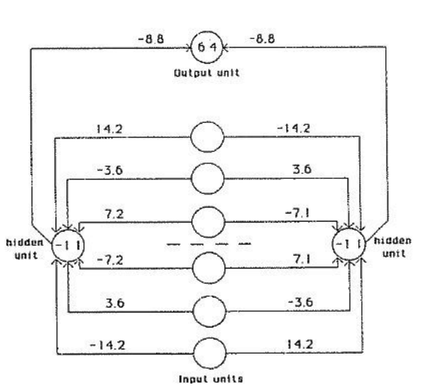
\includegraphics[width=0.55\textwidth]{assets/figures/image_rnn.png}
    \caption{A imagem ilustra um sistema simples de ajuste de peso entre os neurônios, \citeonline{Rumelhart1986}}
    \label{fig:rumelhart}
\end{figure}

Podendo ser usada para previsão de demanda, classificação de texto, reconhecimento de fala, entre outros. As RNNs são capazes de capturar dependências temporais em dados sequenciais, o que as torna adequadas para tarefas como previsão de séries temporais, onde os padrões podem se estender por longos intervalos de tempo. No entanto, as RNNs tradicionais enfrentam dificuldades para aprender dependências de longo prazo devido ao problema do desvanecimento do gradiente, o que limita sua eficácia em tarefas que exigem a retenção de informações por períodos prolongados.

A arquitetura Long Short-Term Memory (LSTM) é um tipo de RNN projetada para lidar com o problema do desvanecimento do gradiente, permitindo que a rede aprenda dependências de longo prazo em dados sequenciais \citeonline{Hochreiter1997}. Diferentemente de uma RNN tradicional, cada célula LSTM mantém um estado de célula (cell state), uma memória de longo prazo que percorre a sequência e cujo conteúdo é regulado por três mecanismos de controle de fluxo denominados portas (gates): a porta de entrada (input gate), que define quais novas informações são incorporadas ao estado de célula; a porta de esquecimento (forget gate), que determina quais informações do estado anterior devem ser descartadas; e a porta de saída (output gate), que controla qual parcela do estado é exposta como saída da célula no instante corrente.

\begin{figure}[H]
    \centering
    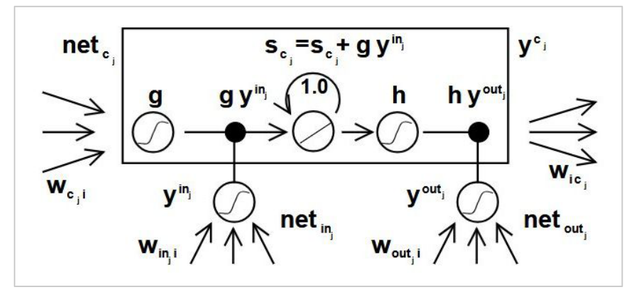
\includegraphics[width=0.7\textwidth]{assets/figures/image_lstm.png}
    \caption{Simples ilustração da arquitetura LSTM, representando a estrutura de memória e os mecanismos de controle de fluxo, \citeonline{Hochreiter1997}}
    \label{fig:lstmcell}
\end{figure}

É essa regulação seletiva manter, atualizar ou descartar informações que permite à LSTM preservar dependências por períodos prolongados sem que o gradiente se dissipe ao longo do tempo, tornando-a especialmente adequada a tarefas como a previsão de séries temporais, nas quais os padrões podem se estender por longos intervalos. Cabe registrar que a formulação original \citeonline{Hochreiter1997} contemplava apenas as portas de entrada e de saída, tendo a porta de esquecimento sido introduzida posteriormente por \citeonline{Gers2000}, configuração que corresponde à forma da arquitetura amplamente utilizada na atualidade. No domínio deste estudo, a previsão de demanda de imunobiológicos, essa capacidade de capturar padrões temporais complexos é crucial para melhorar a precisão das previsões e otimizar o gerenciamento de suprimentos.

\subsection{Previsão de Ruptura e Níveis de Estoque}
\label{subsec:ruptura}

A previsão de ruptura de estoque (stockout), refere-se à antecipação do momento em que o nível de um item disponível torna-se insuficiente para atender à demanda. No contexto da imunização, esse evento é particularmente crítico, pois a ausência do imunobiológico na sala de vacinação resulta em oportunidades de vacinação perdidas e na redução da cobertura vacinal \cite{Lopes2022}. Para mitigar esse risco, a literatura de gestão de operações estabelece dois conceitos fundamentais que orientam a política de reposição: o estoque de segurança (safety stock), entendido como a quantidade adicional mantida em estoque para absorver variações na demanda e nos prazos de entrega, e o ponto de pedido (reorder point), definido como o nível de estoque a partir do qual uma nova ordem de reposição deve ser emitida, calculado tradicionalmente como a soma entre a demanda esperada durante o tempo de espera e o estoque de segurança. A precisão desses parâmetros depende diretamente da qualidade da previsão de demanda subjacente, uma vez que estimativas imprecisas geram tanto excesso de estoque, com custos financeiros e risco de vencimento, quanto rupturas, com prejuízos operacionais e clínicos.

Tradicionalmente, esses cálculos têm sido realizados por meio de fórmulas estatísticas que assumem distribuições conhecidas da demanda e do tempo de espera, o que pode ser limitante em cadeias de saúde marcadas por demandas intermitentes, sazonalidades, campanhas e eventos epidemiológicos. Para superar essas restrições, estudos recentes têm proposto integrar modelos de aprendizado profundo, especialmente arquiteturas recorrentes como a LSTM, ao processo de previsão de demanda que alimenta o cálculo do estoque de segurança e do ponto de pedido. Trabalhos como o de \citeonline{SEYEDAN2023100024} demonstram que abordagens baseadas em Aprendizado em Conjunto (ensemble) com LSTM podem melhorar a acurácia das previsões e, consequentemente, permitir a definição dinâmica dos níveis de estoque sob diferentes cenários de tempo de espera. Entretanto, conforme apontam \citeonline{math14050838}, em séries com baixa razão sinal-ruído, modelos LSTM treinados com função de perda quadrática, Erro Quadrático Médio (MSE), tendem a suavizar picos de demanda, o que pode resultar em subestimação sistemática e em cálculos enviesados do estoque de segurança, aumentando o risco de ruptura. Esse comportamento reforça a necessidade de avaliar não apenas a acurácia média do modelo, mas também sua sensibilidade frente a variações nas entradas, especialmente quando suas previsões alimentam decisões logísticas com impacto direto sobre a operação da rede de imunização.

\subsection{Análise de Sensibilidade e Robustez em Modelos de IA}
\label{subsec:sensibilidade}

A análise de sensibilidade em modelos de inteligência artificial consiste no estudo sistemático de como variações controladas em parâmetros ou entradas do modelo afetam suas saídas, sendo um instrumento essencial para avaliar a estabilidade, a interpretabilidade e a confiabilidade de soluções baseadas em aprendizado profundo. No contexto de redes neurais, essa análise pode ser conduzida em duas frentes principais: a sensibilidade a hiperparâmetros, que examina o impacto de escolhas estruturais, como número de camadas, taxa de aprendizado, função de ativação e dimensão de janela temporal sobre o desempenho preditivo \citeonline{novello2022}; e a sensibilidade aos dados de entrada, que avalia a resposta do modelo frente a perturbações aplicadas às variáveis da série temporal, sejam elas ruídos, valores faltantes ou alterações em variáveis específicas \citeonline{wang2024}. Já o conceito de robustez é frequentemente associado à capacidade do modelo de manter desempenho estável diante dessas perturbações, sendo, portanto, uma propriedade verificada a partir da análise de sensibilidade. Em séries temporais, essas avaliações são particularmente relevantes, pois pequenas variações em parâmetros como tamanho da janela de entrada ou taxa de regularização podem alterar significativamente a capacidade do modelo de capturar padrões temporais complexos.

Entre as técnicas mais utilizadas para conduzir esse tipo de análise, destacam-se métodos baseados em perturbação direta das entradas com medição da variação na saída, conforme descrito por \citeonline{guan2024}, índices estatísticos como o critério HSIC (Hilbert-Schmidt Independence Criterion) aplicado à exploração do espaço de hiperparâmetros, conforme citado por \citeonline{novello2022}, e abordagens de explicabilidade como SHAP e LIME (Seção~\ref{subsec:shap_lime}). Quando aplicadas a modelos LSTM, essas técnicas permitem identificar quais janelas temporais e quais variáveis exercem maior influência sobre a previsão, fornecendo subsídios para a interpretação e o aprimoramento do modelo, conforme explicado por \citeonline{Divyani2025}. Além disso, estudos de ablação, em que componentes do modelo ou subconjuntos de features são removidos para observar o impacto no desempenho, complementam a avaliação ao expor possíveis dependências críticas. No contexto da previsão de demanda de imunobiológicos, a aplicação dessas técnicas é especialmente pertinente, pois os registros de vacinação costumam apresentar ruídos, digitação tardia, registros incompletos e padrões irregulares decorrentes de campanhas e de eventos epidemiológicos, fatores que tornam a análise de sensibilidade um requisito tanto técnico quanto operacional para garantir confiabilidade nas decisões logísticas baseadas no modelo.

\subsection{Explicabilidade: SHAP e LIME}
\label{subsec:shap_lime}

SHAP (SHapley Additive exPlanations) é um método de atribuição de importância baseado nos valores de Shapley da teoria dos jogos cooperativos, que explica a previsão de um modelo como a soma da contribuição de cada variável de entrada em relação a um valor de referência \cite{Lundberg2017}. Os valores de Shapley têm propriedades desejáveis, como a aditividade e a consistência, que dão às atribuições um respaldo teórico. Para modelos arbitrários, como redes recorrentes, utiliza-se o KernelExplainer, que aproxima esses valores por meio de uma regressão linear ponderada sobre amostras de coalizões de variáveis, a um custo computacional que cresce com o número de variáveis e com o tamanho do conjunto de referência.

LIME (Local Interpretable Model-agnostic Explanations) explica a previsão de uma amostra ajustando, na vizinhança dela, um modelo interpretável, em geral linear, às respostas do modelo original sobre versões perturbadas da amostra, ponderadas por sua proximidade \cite{Ribeiro2016}. Os coeficientes do modelo local indicam quais variáveis mais influenciam aquela previsão. Por ser uma explicação local, depende da definição da vizinhança e da amostragem das perturbações, o que pode torná-la instável entre execuções.

Ambas as técnicas independem da arquitetura do modelo e produzem atribuições por amostra, que podem ser agregadas, por exemplo pela média dos valores absolutos, para estimar uma importância global. Como se baseiam em princípios distintos, a concordância entre elas fortalece a leitura de uma atribuição, e a divergência sinaliza que ela deve ser interpretada com cautela. Por isso são usadas em conjunto neste trabalho (Seção~\ref{subsec:impl_explicabilidade}), com cada mês da janela temporal tratado como uma variável.

\subsection{Pré-processamento de Séries Temporais e Imputação de Dados}
\label{subsec:preprocessamento}

O pré-processamento de séries temporais compreende um conjunto de etapas fundamentais que precedem a modelagem preditiva, incluindo normalização, verificação de estacionariedade, remoção de outliers e decomposição da série em seus componentes estruturais. Em séries temporais reais, a não estacionariedade é um desafio recorrente, uma vez que propriedades estatísticas como média e variância variam ao longo do tempo, dificultando a generalização de modelos de aprendizado profundo, como citado por \citeonline{Wang2026survey}. Técnicas como diferenciação, decomposição sazonal e normalização por instância têm sido amplamente utilizadas para mitigar esses efeitos, permitindo que os modelos capturem padrões temporais com maior fidelidade. A decomposição STL (Seasonal-Trend decomposition using LOESS) destaca-se por sua versatilidade e robustez, sendo aplicada como etapa de pré-processamento em combinação com modelos de aprendizado de máquina para melhorar o desempenho preditivo, como demonstrado em \citeonline{Bandara2021}.

A imputação de dados ausentes é etapa crítica no tratamento de séries temporais, especialmente em contextos onde falhas de registro eletrônico são frequentes. Relações temporais são afetadas quando valores ausentes são simplesmente ignorados, pois padrões sazonais podem ser obscurecidos, tornando imprescindível a adoção de estratégias de imputação mais sofisticadas, mostrado por \citeonline{Poette2026}. Além das abordagens tradicionais como média, mediana e LOCF (last observation carried forward), modelos de aprendizado profundo têm demonstrado crescente capacidade para imputação de séries temporais multivariadas, com redes neurais recorrentes e arquiteturas baseadas em Transformers se destacando nos benchmarks recentes, demonstrado em \citeonline{Wang2025imputation}. A escolha do método de imputação deve considerar o mecanismo de ausência dos dados (MCAR, MAR ou MNAR) e a estrutura temporal da série, pois abordagens inadequadas podem introduzir viés sistemático nos resultados, demonstrado por \citeonline{Haneuse2021}.

\subsection{Métricas de Desempenho e Erro}
\label{subsec:metricas}

A avaliação quantitativa de modelos preditivos em séries temporais depende da escolha criteriosa de métricas de erro que reflitam adequadamente a natureza do problema. As métricas mais comuns incluem o Erro Absoluto Médio (MAE), a Raiz do Erro Quadrático Médio (RMSE) e o Erro Percentual Absoluto Médio (MAPE): o RMSE é preferido quando erros maiores devem ser penalizados com mais intensidade, enquanto o MAPE expressa o erro como percentual dos valores reais, facilitando a comparação entre séries de diferentes escalas, como citado em \citeonline{Makridakis2022}. Cada métrica apresenta limitações específicas: o MAPE é problemático quando os valores reais se aproximam de zero, situação frequente em demandas intermitentes, e apresenta assimetria ao penalizar mais fortemente as superestimações do que as subestimações.

O MASE (Erro Médio Absoluto Escalonado) tem ganhado espaço como alternativa robusta, especialmente por sua capacidade de comparar desempenhos entre séries de diferentes escalas sem ser afetado por valores nulos, sendo considerado superior ao benchmark ingênuo quando seu valor é inferior a 1, citado em \citeonline{Makridakis2022}. Em contextos aplicados à saúde, a escolha da métrica deve também considerar as implicações operacionais dos erros: superestimações e subestimações da demanda em saúde têm custos assimétricos, o excesso de provisão gera desperdício de recursos, enquanto a subestimação compromete a qualidade do atendimento \citeonline{Vollmer2021}. A avaliação de precisão não deve se restringir à etapa final da modelagem, mas estar integrada ao longo de todo o fluxo de trabalho, incluindo seleção de modelos, ajuste de hiperparâmetros e monitoramento contínuo em produção.

\subsubsection{Erro Absoluto Médio (MAE)}
\label{subsec:mae}

\begin{equation}
\text{MAE} = \frac{1}{n}\sum_{i=1}^{n}\left|y_i - \hat{y}_i\right|
\end{equation}

Mede a média dos valores absolutos dos erros, onde $y_i$ é o valor real, $\hat{y}_i$ é o valor previsto e $n$ é o número de observações. Por usar o valor absoluto, todos os erros têm o mesmo peso, independentemente do sinal. O resultado fica na mesma unidade da variável original, o que facilita a interpretação. É robusto a outliers, já que não eleva os erros ao quadrado.

\subsubsection{Raiz do Erro Quadrático Médio (RMSE)}
\label{subsec:rmse}

\begin{equation}
\text{RMSE} = \sqrt{\frac{1}{n}\sum_{i=1}^{n}\left(y_i - \hat{y}_i\right)^2}
\end{equation}

É a raiz quadrada da média dos erros elevados ao quadrado. Como os erros são elevados ao quadrado antes de serem somados, o RMSE penaliza mais fortemente os erros grandes, ou seja, é mais sensível a outliers do que o MAE. A raiz quadrada final devolve o resultado à mesma unidade da variável original. Sempre vale a relação RMSE $\geq$ MAE.

\subsubsection{Erro Percentual Absoluto Médio (MAPE)}
\label{subsec:mape}

\begin{equation}
\text{MAPE} = \frac{100\%}{n}\sum_{i=1}^{n}\left|\frac{y_i - \hat{y}_i}{y_i}\right|
\end{equation}

Expressa o erro como uma porcentagem média em relação aos valores reais, o que o torna adimensional e útil para comparar o desempenho entre conjuntos de dados de escalas diferentes. Tem duas limitações importantes: fica indefinido quando algum $y_i = 0$ e tende a penalizar de forma assimétrica, pesando mais as previsões que superestimam do que as que subestimam.

\subsubsection{Erro Absoluto Escalado Médio (MASE)}
\label{subsec:mase}

Para a fórmula, precisamos definir duas quantidades. O erro do modelo no instante $i$ é:

\begin{equation}
e_i = y_i - \hat{y}_i
\end{equation}

E o erro médio absoluto do preditor ingênuo sazonal (naive com período $m$), calculado in-sample sobre $T$ observações de treinamento, é:

\begin{equation}
\text{MAE}_{\text{naive}} = \frac{1}{T-m}\sum_{t=m+1}^{T}\left|y_t - y_{t-m}\right|
\end{equation}

O MASE é então definido como \cite{Hyndman2006}:

\begin{equation}
\text{MASE} = \frac{1}{n}\sum_{i=1}^{n}\frac{\left|e_i\right|}{\text{MAE}_{\text{naive}}} = \dfrac{\dfrac{1}{n}\displaystyle\sum_{i=1}^{n}\left|y_i - \hat{y}_i\right|}{\dfrac{1}{T-m}\displaystyle\sum_{t=m+1}^{T}\left|y_t - y_{t-m}\right|}
\end{equation}

onde $m$ é o período sazonal da série e $T$ é o número de observações de treinamento. Por ser adimensional e normalizado por um benchmark bem definido, o MASE resolve as duas limitações centrais do MAPE: permanece definido mesmo quando $y_i = 0$, o que é relevante neste trabalho, uma vez que municípios de pequeno porte podem registrar zero doses aplicadas de determinado imunobiológico em alguns meses, e não apresenta a assimetria de penalização observada naquela métrica. Um valor MASE $<$ 1 indica que o modelo supera o preditor ingênuo sazonal; um valor MASE $>$ 1 indica desempenho inferior a ele.

\subsection{Particularidades da Demanda por Imunobiológicos}
\label{subsec:particularidades}

A demanda por imunobiológicos, expressa pelo número de doses aplicadas, apresenta características estruturais que a distinguem de outras séries de consumo em saúde. Diferentemente da demanda hospitalar por medicamentos, fortemente associada a eventos agudos, a aplicação de vacinas resulta da sobreposição de três processos geradores. O primeiro é a vacinação de rotina, definida pelo Calendário Nacional de Vacinação e vinculada a marcos etários, como as doses de BCG e de hepatite B indicadas ao nascer \cite{BrasilCalendario2026}, o que aproxima a demanda dessas vacinas do número de nascimentos em cada localidade. O segundo são as campanhas, das quais a vacinação anual contra a influenza é o exemplo mais característico: sua realização antecede o período de maior circulação dos vírus respiratórios, concentrado tipicamente no outono e no inverno, ainda que com variações regionais relevantes \cite{SBIm2026}, e produz picos sazonais pronunciados nas séries. O terceiro são as decisões de política pública que alteram o público-alvo ou o número de doses de um esquema, como a adoção da dose única da vacina contra o HPV para pessoas de 9 a 14 anos em 2024 \cite{BrasilNT412024}.

Do ponto de vista da modelagem, cada um desses processos impõe desafios distintos. As alterações de esquema vacinal e de público-alvo configuram pontos de mudança, isto é, mudanças abruptas de patamar em séries não estacionárias, fenômeno que \citeonline{Xu2025} identificaram afetar parcela expressiva dos itens de maior movimentação em uma farmácia hospitalar. O período de 2020 e 2021, marcado pela pandemia de COVID-19 e pela reorganização dos serviços de saúde, constitui outro potencial ponto de mudança, a ser verificado na análise exploratória dos dados.

Há ainda particularidades relacionadas à qualidade dos registros. A digitação das doses aplicadas pode ocorrer com atraso em relação à data da vacinação, e é comum que pessoas sejam vacinadas em município diferente daquele em que residem, o que pode gerar inconsistências quando os dados são agregados geograficamente \cite{Lopes2022}. Esses fatores introduzem ruídos e lacunas nas séries e reforçam a pertinência de avaliar a sensibilidade do modelo a perturbações nos dados de entrada.

\subsection{O Programa Nacional de Imunizações e os imunobiológicos selecionados}
\label{subsec:pni}

A partir de 2020, os registros de vacinação do SI-PNI passaram a ser disponibilizados de forma individualizada, com um registro por dose aplicada \cite{BrasilPNIDados}. Esses microdados, anonimizados, são publicados pelo Ministério da Saúde no portal OpenDataSUS e por meio de sua API de dados abertos, e contemplam informações sobre a vacina aplicada, a data de aplicação, o estabelecimento de saúde e características demográficas do vacinado. Essa granularidade permite construir séries temporais de demanda em diferentes níveis de agregação, mas exige uma etapa de pré-processamento considerável, descrita na Seção~\ref{sec:conjunto_dados}.

Neste trabalho, foram selecionados quatro imunobiológicos: BCG, hepatite B, influenza e HPV. A escolha busca reunir, em um mesmo estudo, séries com processos geradores distintos (Seção~\ref{subsec:particularidades}): a BCG representa a vacinação de rotina em dose única ao nascer; a hepatite B combina a dose ao nascer com esquemas destinados a adolescentes e adultos não vacinados \cite{BrasilCalendario2026}; a influenza representa a demanda sazonal dirigida por campanhas anuais; e o HPV representa uma série sujeita a mudanças de política, como a adoção da dose única em 2024 \cite{BrasilNT412024}. O recorte geográfico abrange o estado de São Paulo, unidade federativa de grande porte e com o maior número de municípios e de doses aplicadas do país, o que fornece séries municipais em número suficiente para o treinamento de um modelo global e com ampla variação de volume entre a capital e os municípios de pequeno porte.

Essa diversidade de padrões é especialmente adequada aos objetivos deste trabalho. A presença simultânea de séries regulares, sazonais e sujeitas a quebras estruturais cria um cenário no qual arquiteturas recorrentes como a LSTM (Seção~\ref{subsec:rnn_lstm}) podem ser avaliadas sob condições variadas, ao mesmo tempo em que expõe o modelo a perturbações, ruídos e registros incompletos, os quais motivam a análise de sensibilidade proposta. Dessa forma, o recorte adotado não apenas delimita o escopo do estudo, como também oferece um cenário realista e desafiador para avaliar a robustez do modelo frente a variações em seus parâmetros de entrada.

\section{Técnicas, métodos ou abordagens existentes}
\label{sec:tecnicas_existentes}

Os trabalhos analisados nesta pesquisa recorrem a abordagens distintas para a previsão de demanda e de séries temporais: modelagem econométrica combinada a aprendizado profundo no setor farmacêutico \cite{SIERRAESPINEL20252791}, redes RNN e LSTM aplicadas a séries financeiras \cite{AGARWAL2024979} e comparação de arquiteturas recorrentes simples e híbridas \cite{YUNITA2025103462}. A Tabela~\ref{tab:abordagens} sintetiza essas abordagens e suas limitações principais.

\begin{table}[htb]
  \centering
  \caption{Comparativo de abordagens relacionadas}
  \label{tab:abordagens}
  \begin{tabular}{p{4cm}p{3.6cm}p{5.4cm}}
    \toprule
    Abordagem & Domínio & Limitação principal \\
    \midrule
    ARIMA + aprendizado profundo (MLOps) & Demanda farmacêutica & Sem análise de sensibilidade \\
    RNN e LSTM & Cotações de ações & Sem análise de sensibilidade; domínio financeiro \\
    RNN, LSTM, GRU e modelos híbridos & Séries de astronomia, saúde e maquinaria & Poucos conjuntos de dados; sem perturbações na entrada \\
    \bottomrule
  \end{tabular}
  \legend{Fonte: Elaborado pelo autor (2026)}
\end{table}

\section{Trabalhos correlatos e limitações}
\label{sec:trabalhos_relacionados}

\subsection{Metodologia da pesquisa bibliográfica}
\label{sec:metodologia_pesquisa}

A seguir são apresentados os principais tópicos que nortearam a condução desta pesquisa:

\begin{itemize}
    \item \textbf{Bases de dados consultadas}: Google Scholar, IEEE Xplore, ACM Digital Library, SciELO, Periódicos CAPES, entre outras;
    \item \textbf{Palavras-chave utilizadas}:
    \begin{itemize}
        \item ("critical inventory" OR "critical stock" OR "medical supplies" OR "hospital formulary") AND ("deep learning" OR "neural network" OR "LSTM" OR "RNN") AND ("forecasting" OR "optimization" OR "demand prediction") AND ("hospital" OR "healthcare" OR "pharmaceutical");
        \item ("LSTM" OR "GRU" OR "recurrent neural network") AND ("time series forecasting" OR "sequential prediction");
        \item ("inventory management" OR "stock forecasting" OR "demand prediction") AND ("hospital" OR "pharmacy" OR "medical supplies" OR "critical stock");
        \item ("sensitivity analysis" OR "feature importance" OR "SHAP" OR "Sobol index" OR "ablation study") AND ("neural network" OR "deep learning" OR "machine learning");
        \item ("vaccine" OR "immunization" OR "immunobiological") AND ("demand forecasting" OR "utilization forecasting") AND ("machine learning" OR "deep learning" OR "LSTM").
    \end{itemize}
    \item \textbf{Critérios de inclusão e exclusão}: Os critérios de inclusão adotados para a seleção dos trabalhos foram: publicações nos idiomas português e inglês; trabalhos do tipo científico, como artigos, dissertações, notícias; publicações dos últimos 5 a 6 anos, garantindo a atualidade das referências; e relevância acadêmica, priorizando trabalhos publicados em periódicos indexados, alinhados à temática central da pesquisa;
    \item \textbf{Período de abrangência}: média de 5 a 6 anos.
\end{itemize}

A pesquisa bibliográfica foi realizada nas bases Google Scholar, IEEE Xplore, ACM Digital Library, SciELO e Periódicos CAPES, entre outras, utilizando combinações de palavras-chave estruturadas em quatro eixos temáticos: gestão de estoques e cadeias de suprimento em saúde, incluindo a de imunobiológicos, redes neurais recorrentes e aprendizado profundo, previsão de demanda em ambientes de saúde, e análise de sensibilidade em modelos de aprendizado de máquina. Entre as expressões empregadas destacam-se termos como "critical inventory", "LSTM", "demand prediction", "hospital pharmacy", "vaccine demand forecasting", "SHAP" e "LIME", combinados por operadores booleanos para maior precisão na recuperação dos resultados. Foram selecionados artigos publicados predominantemente nos últimos cinco a seis anos, em português e inglês, que abordassem diretamente a aplicação de técnicas de aprendizado profundo com ênfase em arquiteturas recorrentes como LSTM e GRU na previsão e otimização de estoques críticos em contextos hospitalares, farmacêuticos e de imunização. Foram excluídos trabalhos que não apresentassem relação direta com os temas centrais da pesquisa, publicações sem revisão por pares e estudos cujo foco recaísse exclusivamente sobre domínios clínicos sem interface com gestão de suprimentos ou modelagem preditiva.

\subsection{Trabalhos selecionados}

Nesta seção serão apresentados 3 trabalhos selecionados que têm como base o uso de redes neurais recorrentes (RNN/LSTM), aprendizado de máquina e séries temporais, além da análise crítica de seus respectivos resultados. Os trabalhos foram escolhidos seguindo os critérios citados em \ref{sec:metodologia_pesquisa}, contribuindo para a compreensão do estado da arte na área. A seguir, é apresentado um resumo individual de cada um dos trabalhos pesquisados, descrevendo seus objetivos, metodologias adotadas e os principais desafios enfrentados ao longo de seu desenvolvimento.

\subsubsection{Trabalho 1: Applying Deep Learning and Forecasting Techniques to the Pharmaceutical Supply Chain}

\citeonline{SIERRAESPINEL20252791} abordou o problema de melhorar o atendimento aos pacientes através da disponibilidade de medicamentos, como também contribuir para a eficácia operacional no setor da saúde. Para resolvê-lo, os autores propuseram aplicar técnicas de modelação econométrica e estratégias de aprendizagem profunda (DL), com o objetivo de mensurar e gerar previsões com uma boa precisão. A metodologia utilizada foi MLOps (Operações de Aprendizagem Automática), abrangendo princípios de desenvolvimento de software com práticas de gestão de sistemas, onde foi usado para identificação de modelos e estratégias mais adequadas. Já para o modelo econométrico ARIMA, foram utilizados critérios como o Critério de Informação de Akaike (AIC), o Critério de Informação Bayesiano (BIC) e o Critério de Informação de Hannan-Quinn (HQIC), em conjunto ao teste de Ljung-Box. E para avaliar o aprendizado profundo, foram usados o Erro Absoluto Médio (MAE), o Erro Quadrático Médio (MSE) e o Raiz do Erro Quadrático Médio (RMSE).

% TODO(Gabriel): substituir a frase abaixo pelos valores numéricos exatos (MAE, MSE, RMSE, AIC, BIC, HQIC) publicados na tabela de resultados de \citeonline{SIERRAESPINEL20252791}, para permitir comparação direta com os resultados deste trabalho.
Os resultados mostraram que os dois modelos, o econométrico ARIMA e o de aprendizado profundo (DL), possuem uma eficácia significativa para previsões de demanda de medicamentos, onde em conjunto podem oferecer uma maior precisão nas previsões, resultado demonstrado com o uso dos critérios definidos. No entanto, a solução apresenta limitações como a ausência de análise de sensibilidade nos parâmetros de entrada e a não avaliação da robustez dos modelos frente a perturbações nos dados de entrada. O presente trabalho diferencia-se por fazer uso de uma base pública de doses aplicadas do PNI, tratada para compor séries mensais por município e imunobiológico, e por aplicar testes nos parâmetros de entrada para avaliar como o modelo de aprendizagem de máquina se comporta frente a essas variações.

\subsubsection{Trabalho 2: Predictive Data Analysis: Leveraging RNN and LSTM Techniques for Time Series Dataset}

\citeonline{AGARWAL2024979} abordou o problema de prever valores futuros de cotações no mercado de ações. Para resolvê-lo, os autores propuseram utilizar Redes Neurais Recorrentes (RNN) e Memória de Longo Prazo (LSTM) para gerar previsões a partir de um conjunto de dados, superando o problema do desvanecimento do gradiente com o uso da arquitetura LSTM. A metodologia utilizada foi estruturar a solução em módulos e classes, sendo eles:
\begin{itemize}
\item Módulo de pré-processamento de dados: inclui as funções para carregar, limpar e normalizar os dados relativos aos preços das ações;
\item Módulo de arquitetura do modelo: inclui as funções para construir os modelos RNN e LSTM;
\item Módulo de treino: inclui as funções para treinar os modelos com base nos dados históricos;
\item Módulo de previsão: inclui as funções para efetuar previsões sobre os dados de teste e avaliar o desempenho dos modelos.
\end{itemize}
Para construir os modelos, os autores utilizaram Python e as bibliotecas Keras e TensorFlow. Para normalizar os dados, foi utilizado o MinMaxScaler da biblioteca sklearn. A separação dos conjuntos de treino e teste foi de 85:15, ou seja, 85\% dos dados foram utilizados para treinar o modelo LSTM e 15\% para teste, com janelas de 100 pontos de dados. O Raiz do Erro Quadrático Médio (RMSE), as medidas R² e as métricas de acurácia foram utilizados para avaliar o desempenho dos modelos.

Os resultados mostraram que o modelo LSTM apresentou desempenho superior ao modelo RNN: o modelo RNN, após 100 épocas, obteve uma acurácia de 97,12\% nos dados de treino e de 81,01\% nos dados de teste, enquanto o modelo LSTM, aplicado ao mesmo conjunto de dados, alcançou 98,10\% nos dados de treino e 91,97\% nos dados de teste. No entanto, assim como o trabalho anterior, a solução apresenta limitações como a ausência de análise de sensibilidade nos parâmetros de entrada, a não avaliação da robustez dos modelos frente a perturbações nos dados e a aplicação restrita ao domínio financeiro, sem contemplar contextos de saúde. O presente trabalho diferencia-se por aplicar métodos de análise de sensibilidade e avaliação da robustez em um modelo preditivo voltado à previsão de demanda de imunobiológicos.

\subsubsection{Trabalho 3: Performance analysis of neural network architectures for time series forecasting: A comparative study of RNN, LSTM, GRU, and hybrid models}

\citeonline{YUNITA2025103462} abordou o problema de avaliar o desempenho de nove arquiteturas de redes neurais para previsão de séries temporais, nomeadamente RNN, LSTM, GRU, RNN-LSTM, RNN-GRU, LSTM-RNN, GRU-RNN, LSTM-GRU e GRU-LSTM. Para resolvê-lo, os autores propuseram uma avaliação baseada no método de Monte Carlo (MC), com o objetivo de garantir a confiabilidade dos resultados frente à variabilidade decorrente da inicialização aleatória dos pesos. A metodologia utilizada consistiu em selecionar três conjuntos de dados nas áreas da astronomia, cuidados de saúde e maquinaria, realizar uma análise exploratória de dados (EDA) como etapa preliminar de avaliação estatística e de qualidade, implementar as diferentes arquiteturas de redes neurais e, por fim, avaliar os modelos por meio de 100 iterações de Monte Carlo, utilizando as métricas de Erro Absoluto Médio (MAE), Erro Percentual Absoluto Médio (MAPE) e Raiz do Erro Quadrático Médio (RMSE).

Os resultados mostraram que, pelo teste de Friedman, não houve diferença estatisticamente significativa entre as arquiteturas avaliadas. Esse resultado pode ter sido influenciado por fatores como a dimensão limitada da amostra, com apenas três conjuntos de dados para avaliação, e o possível mascaramento das diferenças de desempenho pelo ruído experimental. Ainda assim, os padrões de desempenho consistentes observados em todos os conjuntos de dados sugerem potenciais vantagens práticas para as arquiteturas híbridas baseadas em LSTM, especialmente as configurações LSTM-RNN e LSTM-GRU. No entanto, a solução apresenta limitações como o número reduzido de conjuntos de dados utilizados na avaliação, a ausência de investigação sobre o impacto de perturbações nos parâmetros de entrada sobre o desempenho preditivo e a não aplicação dos modelos à gestão de suprimentos em saúde. O presente trabalho diferencia-se por aplicar uma análise de sensibilidade sistemática nos parâmetros de entrada de um modelo LSTM voltado à previsão de demanda de imunobiológicos, investigando como variações nesses parâmetros afetam o desempenho preditivo, parte não explorada por \citeonline{YUNITA2025103462}, que avaliam a robustez apenas em relação à inicialização aleatória dos pesos, sem considerar perturbações nos dados de entrada.

\subsection{Posicionamento deste trabalho em relação aos correlatos}

Posicionamento acadêmico dos trabalhos relacionados:

\begin{figure}[H]
    \centering
    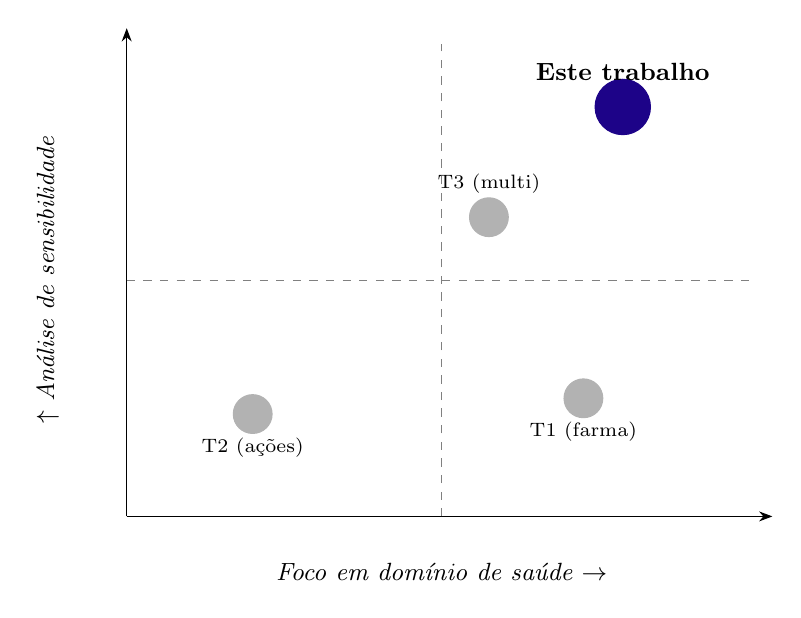
\begin{tikzpicture}[scale=1.0]
        \draw[-Stealth] (0,0) -- (8.2,0);
        \draw[-Stealth] (0,0) -- (0,6.2);
        \draw[dashed, gray] (4,0) -- (4,6);
        \draw[dashed, gray] (0,3) -- (8,3);
        \node[font=\small\itshape] at (4,-0.7) {Foco em domínio de saúde $\rightarrow$};
        \node[font=\small\itshape, rotate=90] at (-1.0,3) {$\uparrow$ Análise de sensibilidade};
        \filldraw[gray!60] (1.6,1.3) circle (7pt);
        \node[font=\scriptsize, below=5pt] at (1.6,1.3) {T2 (ações)};
        \filldraw[gray!60] (5.8,1.5) circle (7pt);
        \node[font=\scriptsize, below=5pt] at (5.8,1.5) {T1 (farma)};
                \filldraw[gray!60] (4.6,3.8) circle (7pt);
        \node[font=\scriptsize, above=5pt] at (4.6,3.8) {T3 (multi)};
        \filldraw[blue!70!black] (6.3,5.2) circle (10pt);
        \node[font=\small\bfseries, above=6pt] at (6.3,5.2) {Este trabalho};
    \end{tikzpicture}
    \caption{A imagem ilustra o posicionamento acadêmico deste trabalho em relação aos trabalhos relacionados}
    \label{fig:posicionamento}
\end{figure}

Uma tabela comparativa ajuda a sintetizar as diferenças entre os trabalhos:

\begin{table}[htb]
    \centering
    \caption{Comparação entre trabalhos relacionados}
    \label{tab:trabalhos_relacionados}

    \footnotesize
    \begin{tabularx}{\textwidth}{>{\raggedright\arraybackslash}p{1.9cm}|>{\raggedright\arraybackslash}X|>{\raggedright\arraybackslash}X|>{\raggedright\arraybackslash}X|>{\raggedright\arraybackslash}X}
        \toprule
        \textbf{Critério} & \textbf{Trabalho 1} & \textbf{Trabalho 2} & \textbf{Trabalho 3} & \textbf{Este trabalho} \\
        \midrule
        Objetivo
        & Previsão de demanda farmacêutica
        & Previsão de cotações de ações
        & Comparação de arquiteturas RNN, LSTM e GRU
        & Análise de sensibilidade de LSTM para demanda de imunobiológicos \\

        \midrule

        Tecnologia
        & ARIMA + DL (MLOps)
        & RNN + LSTM (Keras/TensorFlow)
        & RNN, LSTM, GRU, modelos híbridos
        & LSTM + análise de sensibilidade + SHAP/LIME \\

        \midrule

        Validação
        & MAE, MSE, RMSE, AIC, BIC
        & RMSE, R², acurácia
        & MAE, MAPE, RMSE (Monte Carlo)
        & MAE, RMSE, MAPE e MASE; cinco sementes \\

        \midrule

        Limitação
        & Sem análise de sensibilidade
        & Sem análise de sensibilidade; domínio financeiro
        & Poucos datasets; sem perturbações na entrada
        & Recorte de quatro imunobiológicos e um estado (SP); séries curtas \\

        \midrule
        Métricas
        & AIC, BIC, HQIC, MAE, MSE e RMSE
        & RMSE
        & MAE, MAPE e RMSE
        & MAE, RMSE, MAPE e MASE \\

        \bottomrule
    \end{tabularx}

    \legend{Fonte: Elaborado pelo autor (2026)}
\end{table}

% ===============================================================
% METODOLOGIA
% ===============================================================
\chapter{Metodologia}
\label{cap:metodologia}

\section{Tipo de pesquisa e hipótese}

Adota-se uma abordagem experimental e incremental. O desenvolvimento parte da construção do pipeline de dados e do modelo de referência (baseline); somente após a validação do baseline os experimentos de sensibilidade são executados, um fator por vez a partir da configuração de referência, de modo a isolar o efeito de cada variação. Essa estratégia evita a explosão combinatória de cenários e mantém a interpretabilidade dos resultados, ao custo de não capturar interações entre fatores (Seção~\ref{sec:limitacoes}). O ciclo de trabalho é iterativo: cada experimento é executado, registrado e analisado antes do planejamento do seguinte, em consonância com a recomendação da literatura de integrar a avaliação de desempenho ao longo de todo o fluxo, e não apenas à etapa final.

Por não haver hipótese formal, o critério de sucesso esperado é o descrito na Seção~\ref{sec:hipotese}: MASE do baseline inferior a 1, entendido como critério mínimo.

\section{Procedimentos da abordagem proposta}
\label{sec:procedimentos}

Os procedimentos seguem, em ordem cronológica, as etapas do pipeline experimental ilustrado na Figura~\ref{fig:pipeline}:

\begin{enumerate}
    \item \textbf{Coleta de dados}: obtenção dos microdados de doses aplicadas do PNI (SI-PNI);
    \item \textbf{Pré-processamento}: filtragem, agregação mensal por município e imunobiológico, normalização, construção das janelas temporais (sliding window) e segmentação em treino, validação e teste;
    \item \textbf{Baseline LSTM}: treinamento e validação do modelo de referência, com critério MASE $<$ 1;
    \item \textbf{Experimentos de sensibilidade}: perturbações controladas, um fator por vez a partir da configuração de referência (janela temporal, ruído, dados faltantes e hiperparâmetros);
    \item \textbf{Explicabilidade}: aplicação de SHAP e LIME, com atribuição de importância às variáveis e janelas temporais;
    \item \textbf{Consolidação dos resultados}: tabelas, gráficos e análise comparativa dos cenários.
\end{enumerate}

\section{Ferramentas, tecnologias e ambientes}
\label{subsec:tecnologias}

A implementação foi realizada em linguagem Python, pela maturidade de seu ecossistema para aprendizado de máquina e por sua adoção nos trabalhos relacionados analisados. Para a construção e o treinamento do modelo LSTM, utilizou-se Keras (versão 3.15.1) sobre TensorFlow (versão 2.21.0), como em \citeonline{AGARWAL2024979}. O pré-processamento e o cálculo de métricas apoiam-se nas bibliotecas scikit-learn, pandas e NumPy. Dado o volume dos microdados do PNI, a leitura é realizada arquivo a arquivo, com filtragem dos registros antes da agregação, de modo a viabilizar o processamento em máquina local. As análises de explicabilidade utilizam as bibliotecas SHAP (versão 0.52.0) e LIME (versão 0.2.0.1), e a visualização dos resultados, Matplotlib.

A experimentação foi conduzida em ambiente de máquina local: Intel(R) Core(TM) i5-14600KF (3,50 GHz) CPU; 16,0 GB RAM; NVIDIA GeForce RTX 5060 (8 GB) GPU, com dependências versionadas em arquivo de requisitos e sementes aleatórias fixadas, com operações determinísticas do TensorFlow habilitadas, de modo que a mesma semente produz o mesmo resultado e a variação entre sementes mede apenas o efeito da inicialização, conforme previsto no objetivo específico 3 (Seção~\ref{sec:objetivos_secundarios}).

\section{Procedimentos experimentais e métricas}
\label{sec:proc_experimentais}

Os experimentos de sensibilidade aplicam perturbações controladas sobre o modelo de referência, registrando as métricas resultantes e sua variabilidade. Nos parâmetros de entrada, variam-se o tamanho da janela temporal (3, 6, 9 e 18 meses, contra 12 no baseline), a injeção de ruído gaussiano nas séries (de 0,05 a 0,3 vez o desvio-padrão da série) e a proporção de valores faltantes (10\%, 20\% e 30\% dos meses, preenchidos por interpolação linear). Nos hiperparâmetros estruturais, variam-se a taxa de dropout (0,1; 0,2 e 0,3, contra 0,0), o número de camadas (2 e 3, contra 1), o número de unidades (16, 32 e 128, contra 64) e a taxa de aprendizado ($10^{-4}$, $5\times10^{-4}$ e $5\times10^{-3}$, contra $10^{-3}$). O ruído e os valores faltantes atingem apenas a entrada do modelo; as métricas são sempre calculadas contra a série original. Cada cenário é executado de forma isolada a partir do modelo de referência (estratégia um fator por vez, OFAT) e repetido com cinco sementes aleatórias (42, 7, 123, 2024 e 31337).

O desempenho é calculado sobre o conjunto de teste pelas métricas MAE, RMSE, MAPE e MASE (Seção~\ref{subsec:metricas}), registradas de forma padronizada a cada execução para posterior comparação. Para não confundir efeito da perturbação com sorte de inicialização, uma variação do MASE só é considerada relevante quando sua diferença para o baseline supera duas vezes o desvio-padrão entre sementes do próprio baseline. A Tabela~\ref{tab:plano_experimentos} apresenta o plano de experimentação.

\begin{table}[htb]
  \centering
  \caption{Plano de experimentação}
  \label{tab:plano_experimentos}
  \begin{tabular}{p{3.6cm}p{6.8cm}p{3cm}}
    \toprule
    Experimento & Variável controlada & Métrica principal \\
    \midrule
    Comparação com baseline & Modelo de referência vs. preditor ingênuo sazonal & MASE \\
    Janela temporal & Tamanho do look-back: 3, 6, 9 e 18 meses (baseline: 12) & MAE, RMSE, MAPE, MASE \\
    Ruído & Ruído gaussiano: 0,05; 0,1; 0,2 e 0,3 do desvio da série & MAE, RMSE, MAPE, MASE \\
    Dados faltantes & Proporção de meses faltantes: 10\%, 20\% e 30\% & MAE, RMSE, MAPE, MASE \\
    Hiperparâmetros & Dropout, camadas, unidades e taxa de aprendizado & MAE, RMSE, MAPE, MASE \\
    Variáveis exógenas & Entrada só com doses vs. doses mais nove covariáveis & MAE, RMSE, MAPE, MASE \\
    \bottomrule
  \end{tabular}
  \legend{Fonte: Elaborado pelo autor (2026)}
\end{table}

\section{Critérios de validação}

O baseline é considerado satisfatório quando seu MASE é inferior a 1. A consistência dos resultados é reforçada pela fixação de sementes aleatórias e pela repetição das execuções com cinco sementes.

% ===============================================================
% DESENVOLVIMENTO
% ===============================================================
\chapter{Desenvolvimento / Implementação / Experimentos}
\label{cap:desenvolvimento}

\section{Modelagem e arquitetura}
\label{sec:solucao}

A solução proposta neste trabalho não consiste em um sistema de software voltado ao usuário final, mas em um pipeline experimental reproduzível para treinamento, avaliação e análise de sensibilidade de um modelo de Rede Neural Recorrente com arquitetura Long Short-Term Memory (LSTM) aplicado à previsão de demanda de imunobiológicos do PNI, expressa pelo número mensal de doses aplicadas por município. O objetivo central do pipeline é, a partir de um modelo de referência (baseline), submeter o modelo a perturbações controladas em seus parâmetros de entrada e hiperparâmetros estruturais e mensurar, de forma sistemática, o impacto dessas variações sobre o desempenho preditivo, avaliado pelas métricas MAE, RMSE, MAPE e MASE, e sobre a importância atribuída às variáveis e instantes temporais, avaliada por meio das técnicas de explicabilidade SHAP e LIME.

\subsection{Arquitetura}
\label{subsec:arquitetura}

A solução é organizada de forma modular, de modo que cada etapa do fluxo seja isolada, parametrizável e reexecutável. Os módulos e suas interações são:

\subsubsection{Módulo de aquisição e pré-processamento de dados}

Responsável por obter os microdados de doses aplicadas do PNI (Seção~\ref{sec:conjunto_dados}) e transformá-los em séries temporais aptas ao treinamento. Para isso, realiza a filtragem dos registros válidos e do recorte de imunobiológicos e unidade federativa, a agregação mensal das doses por município e imunobiológico, o preenchimento dos meses sem registro com zero e o cálculo das variáveis exógenas por município, imunobiológico e mês. A normalização (transformação $\log(1+x)$ seguida de padronização por série, com média e desvio calculados apenas sobre os meses de treino) e a construção das janelas temporais (sliding window) são feitas no momento do treinamento. Esse módulo também realiza a segmentação dos dados em conjuntos de treino, validação e teste, respeitando a ordem cronológica das observações.

\subsubsection{Módulo de definição do modelo}

Encapsula a construção da arquitetura LSTM, expondo como parâmetros configuráveis o número de camadas, o número de unidades, a taxa de aprendizado e a taxa de dropout (aplicada tanto às conexões de entrada quanto às conexões recorrentes), de modo a permitir variações controladas nos experimentos posteriores.

\subsubsection{Módulo de treinamento}

Executa o treinamento do modelo a partir dos dados de treino e validação, com controle de épocas, restauração dos pesos da melhor época de validação e fixação de sementes aleatórias para garantir reprodutibilidade.

\subsubsection{Módulo de avaliação}

Calcula as métricas de desempenho (MAE, RMSE, MAPE e MASE) sobre o conjunto de teste, registrando os resultados de cada execução de forma padronizada para posterior comparação.

\subsubsection{Módulo de experimentos de sensibilidade}

Coordena a aplicação das perturbações controladas descritas na Seção~\ref{sec:proc_experimentais}. Cada cenário é executado de forma isolada a partir do modelo de referência, registrando-se as métricas resultantes e sua variabilidade entre as cinco sementes.

\subsubsection{Módulo de explicabilidade}

Aplica as técnicas SHAP e LIME ao modelo treinado, identificando quais variáveis e janelas temporais exercem maior influência sobre as previsões, complementando a análise de sensibilidade por perturbação com uma perspectiva de atribuição.

\subsubsection{Módulo de registro e análise de resultados}

Consolida os resultados de todas as execuções, gera tabelas e visualizações comparativas e dá suporte à discussão sobre quais fatores representam maior risco para a aplicação prática.

A interação entre os módulos segue um fluxo sequencial: os dados pré-processados alimentam o modelo, que é treinado e avaliado para estabelecer o baseline. Em seguida, o módulo de experimentos reexecuta o ciclo sob diferentes perturbações; por fim, os módulos de explicabilidade e de análise consolidam os resultados. Segue uma ilustração do fluxo por meio de um diagrama, demonstrativo na Figura~\ref{fig:pipeline}:

\begin{figure}[H]
    \centering
    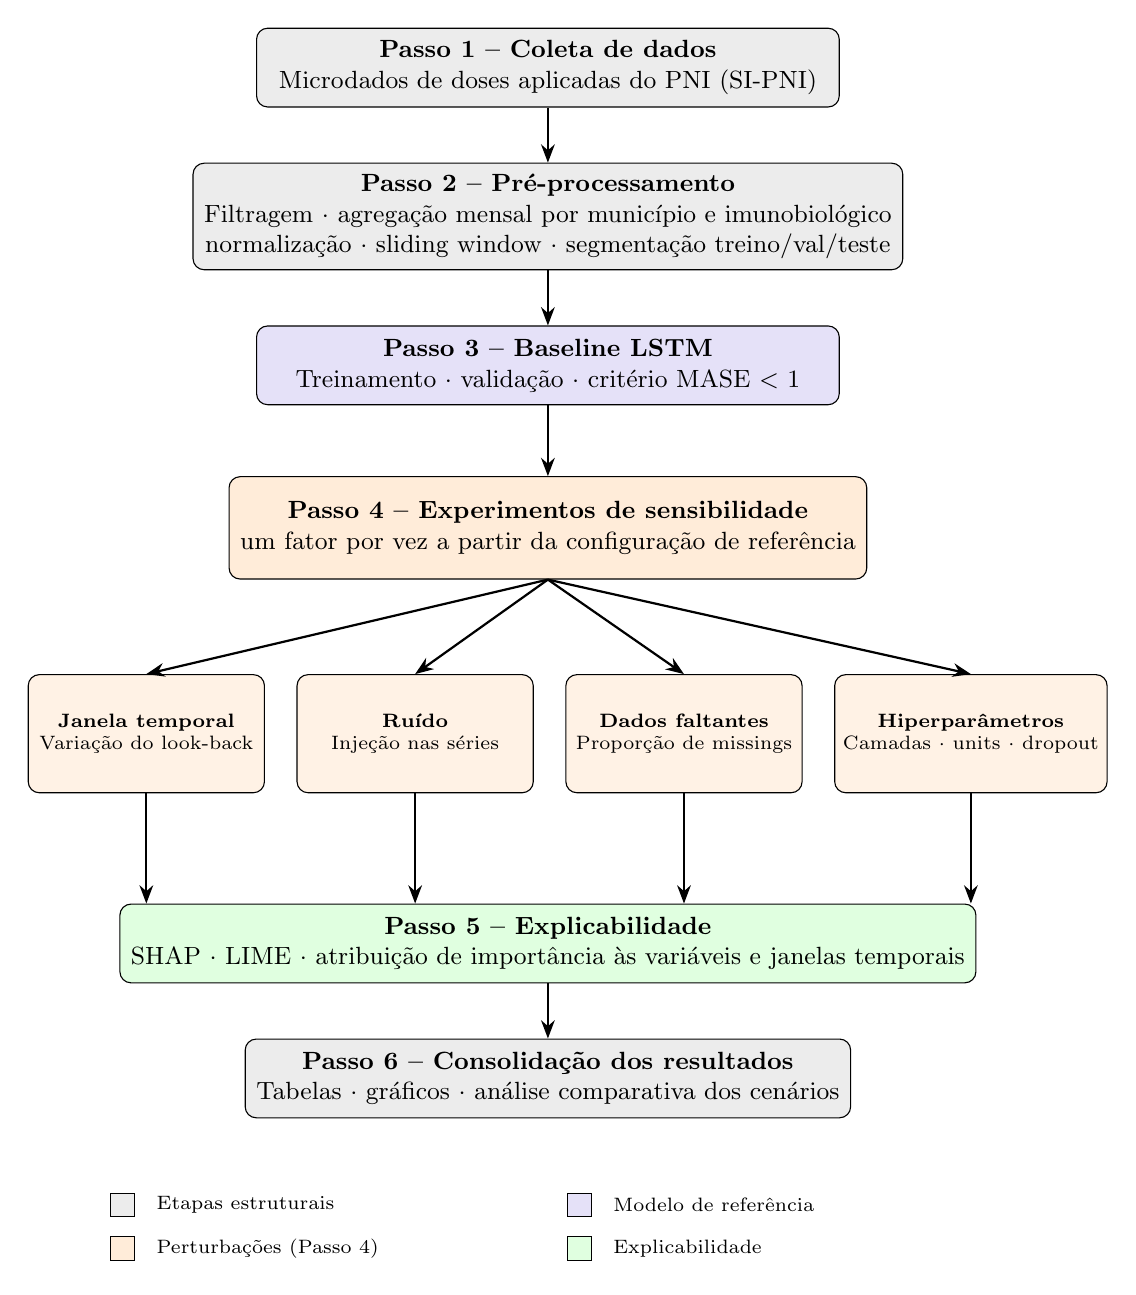
\begin{tikzpicture}[
        node distance=7mm and 6mm,
        box/.style={draw, rounded corners, align=center, minimum width=7.4cm, minimum height=1cm, font=\small, inner sep=4pt},
        subbox/.style={draw, rounded corners, align=center, minimum width=3.0cm, minimum height=1.5cm, font=\scriptsize, inner sep=3pt},
        arr/.style={-Stealth, thick}
    ]
        \node[box, fill=gray!15] (p1) {\textbf{Passo 1 -- Coleta de dados}\\Microdados de doses aplicadas do PNI (SI-PNI)};
        \node[box, fill=gray!15, below=of p1] (p2) {\textbf{Passo 2 -- Pré-processamento}\\Filtragem $\cdot$ agregação mensal por município e imunobiológico\\normalização $\cdot$ sliding window $\cdot$ segmentação treino/val/teste};
        \node[box, fill=blue!12, below=of p2] (p3) {\textbf{Passo 3 -- Baseline LSTM}\\Treinamento $\cdot$ validação $\cdot$ critério MASE $<$ 1};
        \node[box, fill=orange!15, below=9mm of p3, minimum height=1.3cm] (p4) {\textbf{Passo 4 -- Experimentos de sensibilidade}\\um fator por vez a partir da configuração de referência};

        \node[subbox, fill=orange!10, below=1.2cm of p4, xshift=-5.1cm] (janela) {\textbf{Janela temporal}\\Variação do look-back};
        \node[subbox, fill=orange!10, right=4mm of janela] (ruido) {\textbf{Ruído}\\Injeção nas séries};
        \node[subbox, fill=orange!10, right=4mm of ruido] (faltantes) {\textbf{Dados faltantes}\\Proporção de missings};
        \node[subbox, fill=orange!10, right=4mm of faltantes] (hiper) {\textbf{Hiperparâmetros}\\Camadas $\cdot$ units $\cdot$ dropout};

        \node[box, fill=green!12, below=1.4cm of janela.south -| p4] (p5) {\textbf{Passo 5 -- Explicabilidade}\\SHAP $\cdot$ LIME $\cdot$ atribuição de importância às variáveis e janelas temporais};
        \node[box, fill=gray!15, below=of p5] (p6) {\textbf{Passo 6 -- Consolidação dos resultados}\\Tabelas $\cdot$ gráficos $\cdot$ análise comparativa dos cenários};

        \draw[arr] (p1) -- (p2);
        \draw[arr] (p2) -- (p3);
        \draw[arr] (p3) -- (p4);
        \draw[arr] (p4.south) -- (janela.north);
        \draw[arr] (p4.south) -- (ruido.north);
        \draw[arr] (p4.south) -- (faltantes.north);
        \draw[arr] (p4.south) -- (hiper.north);
        \draw[arr] (janela.south) -- (janela.south |- p5.north);
        \draw[arr] (ruido.south) -- (ruido.south |- p5.north);
        \draw[arr] (faltantes.south) -- (faltantes.south |- p5.north);
        \draw[arr] (hiper.south) -- (hiper.south |- p5.north);
        \draw[arr] (p5) -- (p6);

        \coordinate (legAnchor) at ($(p6.south)+(0,-1.1cm)$);
        \node[draw, fill=gray!15, minimum width=0.3cm, minimum height=0.3cm] at ($(legAnchor)+(-5.4cm,0)$) (leg1) {};
        \node[font=\scriptsize, anchor=west] at ($(leg1.east)+(0.15cm,0)$) {Etapas estruturais};
        \node[draw, fill=blue!12, minimum width=0.3cm, minimum height=0.3cm] at ($(legAnchor)+(0.4cm,0)$) (leg2) {};
        \node[font=\scriptsize, anchor=west] at ($(leg2.east)+(0.15cm,0)$) {Modelo de referência};
        \node[draw, fill=orange!15, minimum width=0.3cm, minimum height=0.3cm] at ($(legAnchor)+(-5.4cm,-0.55cm)$) (leg3) {};
        \node[font=\scriptsize, anchor=west] at ($(leg3.east)+(0.15cm,0)$) {Perturbações (Passo 4)};
        \node[draw, fill=green!12, minimum width=0.3cm, minimum height=0.3cm] at ($(legAnchor)+(0.4cm,-0.55cm)$) (leg4) {};
        \node[font=\scriptsize, anchor=west] at ($(leg4.east)+(0.15cm,0)$) {Explicabilidade};
    \end{tikzpicture}
    \caption{Pipeline experimental proposto para análise de sensibilidade do modelo LSTM}
    \label{fig:pipeline}
\end{figure}

\section{Detalhes de implementação}
\label{subsec:funcionalidades}

A implementação em Python utiliza Keras para a construção e o treinamento do modelo LSTM, scikit-learn para métricas, e pandas e NumPy para manipulação de dados (Seção~\ref{subsec:tecnologias}). Dado o volume dos microdados do PNI, a leitura é realizada arquivo a arquivo, mantendo apenas contadores agregados em memória. As janelas temporais são construídas por sliding window, respeitando a ordem cronológica na segmentação em treino, validação e teste, e a taxa de dropout é aplicada tanto às conexões de entrada quanto às recorrentes.

As funcionalidades do pipeline, alinhadas aos objetivos do trabalho, são: treinar e avaliar um modelo LSTM de referência para previsão de demanda de imunobiológicos; executar experimentos de perturbação controlada sobre parâmetros de entrada e hiperparâmetros; mensurar a variabilidade das métricas de desempenho frente a cada perturbação; gerar, por meio de SHAP e LIME, a importância das variáveis e dos instantes temporais nas previsões; e consolidar os resultados em tabelas e gráficos que permitam comparar os cenários e identificar os fatores de maior influência.

\subsection{Modelo de referência e treinamento}
\label{subsec:baseline_config}

A tarefa é formulada como previsão um passo à frente: dadas as doses dos 12 meses anteriores, prevê-se o mês seguinte. Cada previsão usa apenas dados observados, sem realimentar a própria saída, de modo que o erro não se acumula ao longo do horizonte. Em vez de um modelo por município, treina-se um único modelo por imunobiológico com todas as séries municipais em conjunto, o que multiplica o número de amostras de treino disponíveis em relação a séries curtas de 32 meses.

Cada série é transformada por $\log(1+x)$, para comprimir a diferença de escala entre a capital e municípios com uma ou duas doses mensais, e padronizada (média e desvio-padrão) por série, com estatísticas calculadas apenas sobre os meses de treino, evitando vazamento de informação do futuro. A divisão é temporal e nunca aleatória: o treino prevê os meses até dezembro de 2025 (12 amostras por município, com a janela cobrindo 2024), a validação prevê janeiro a abril de 2026 e o teste prevê maio a agosto de 2026. A validação serve apenas para escolher a melhor época.

A arquitetura de referência é composta por uma camada LSTM de 64 unidades, uma camada densa de 32 neurônios com ativação ReLU e uma camada de saída linear. Utilizam-se perda MSE, otimizador Adam com taxa de aprendizado de $10^{-3}$, lotes de 32 amostras e no máximo 80 épocas, restaurando-se ao final os pesos da época de menor perda de validação. O porte reduzido é intencional: o treino conta entre 1.944 e 7.392 amostras por imunobiológico, e um modelo maior tenderia ao sobreajuste. A janela de 12 meses foi definida a priori para cobrir um ciclo anual completo e permitir que o modelo enxergue a sazonalidade. Como o treino cobre apenas 24 meses de histórico, o período sazonal do MASE é $m=12$.

\subsection{Variáveis exógenas}
\label{subsec:exogenas}

Além do modelo que recebe apenas a série de doses, implementou-se uma variante que acrescenta, a cada mês da janela, nove covariáveis calculadas a partir dos próprios microdados por município, imunobiológico e mês: idade média dos vacinados, proporção de doses por faixa etária (0 a 1, 2 a 4, 5 a 19, 20 a 59 e 60 anos ou mais), proporção de doses aplicadas em estabelecimentos públicos, proporção de doses com natureza do estabelecimento desconhecida e uma indicadora de mês sem aplicação. Essas variáveis funcionam como indicadores do público-alvo e do canal de aplicação, que alteram a demanda sem aparecer na série de doses. Nos meses sem doses, a covariável repete o último valor conhecido e a indicadora sinaliza o mês. A covariável do mês previsto nunca entra na janela. Com isso, cada mês da janela passa a ter 10 variáveis (doses mais nove covariáveis), e a janela de 12 meses totaliza 120 entradas.

\subsection{Explicabilidade}
\label{subsec:impl_explicabilidade}

SHAP e LIME foram aplicados ao modelo de referência treinado com a semente 42, sobre 200 amostras do conjunto de teste, tratando cada mês da janela como uma variável ($t\text{-}12$ a $t\text{-}1$, em que $t\text{-}1$ é o mês imediatamente anterior ao previsto). Para o SHAP utilizou-se o KernelExplainer com fundo de 20 centroides obtidos por k-means sobre o treino; para o LIME, um modelo linear local em torno de cada amostra, com 1.000 perturbações e sem discretização, de modo que os pesos sejam comparáveis aos do SHAP. As importâncias foram normalizadas para somar 1, pois as escalas diferem entre as técnicas. No modelo com variáveis exógenas, a importância é apresentada tanto por mês da janela quanto por variável.

\section{Experimentos e cenários de teste}

Os cenários de teste correspondem às perturbações descritas na Seção~\ref{sec:proc_experimentais}, executadas um fator por vez a partir da configuração de referência: tamanho da janela temporal, injeção de ruído nas séries, proporção de valores faltantes e hiperparâmetros estruturais (dropout, número de camadas, número de unidades e taxa de aprendizado). Essa estratégia evita a explosão combinatória de cenários e mantém a interpretabilidade dos resultados. Os conjuntos de dados são as séries mensais dos quatro imunobiológicos no estado de São Paulo (Seção~\ref{sec:conjunto_dados}), e cada configuração é executada com cinco sementes fixadas, de modo a distinguir o efeito das perturbações do ruído decorrente da inicialização do modelo. Os experimentos foram executados para o modelo apenas com doses e, depois, repetidos integralmente para o modelo com variáveis exógenas.

\section{Coleta e tratamento de dados}
\label{sec:conjunto_dados}

A base de dados adotada neste trabalho é composta pelos microdados de doses aplicadas do Programa Nacional de Imunizações, de natureza pública e aberta, disponibilizados pelo Ministério da Saúde por meio do portal OpenDataSUS e de sua API de dados abertos \cite{BrasilPNIDados}. A partir de 2020, cada registro da base corresponde a uma dose aplicada e contém, entre outras informações, a data da vacinação, o código do imunobiológico, o município e a unidade federativa do estabelecimento de saúde, características anonimizadas do vacinado, como idade e sexo, e campos de controle do registro, como sua situação e eventual exclusão. A base foi selecionada por sua disponibilidade aberta, por sua abrangência nacional e pela continuidade das séries, fatores que conferem validade e reprodutibilidade aos resultados obtidos, além de representar diretamente o consumo de imunobiológicos na ponta da cadeia de suprimentos.

Com o objetivo de concentrar a análise em um conjunto de séries representativo dos diferentes padrões de demanda discutidos na Seção~\ref{subsec:particularidades}, o recorte adotado contempla os quatro imunobiológicos apresentados na Tabela~\ref{tab:imunobiologicos}, aplicados em estabelecimentos de saúde do estado de São Paulo.

% Códigos conferidos na documentação de regras de validação de vacinação do e-SUS APS
% (integracao.esusaps.bridge.ufsc.tech/ledi/documentacao/regras/validar_regras_vacinacao.html):
% 9 = vacina hepatite B; 15 = vacina BCG; 33 = vacina influenza trivalente; 67 = vacina HPV quadrivalente.
\begin{table}[htb]
    \centering
    \caption{Imunobiológicos selecionados}
    \label{tab:imunobiologicos}
    \begin{tabularx}{\textwidth}{l|c|>{\raggedright\arraybackslash}X}
        \toprule
        \textbf{Imunobiológico} & \textbf{Código (\texttt{codigo\_vacina})} & \textbf{Padrão de demanda predominante} \\
        \midrule
        BCG & 15 & Rotina; dose única ao nascer \\
        Hepatite B & 9 & Rotina ao nascer e esquemas para adolescentes e adultos não vacinados \\
        Influenza & 33 & Sazonal; campanha anual \\
        HPV & 67 & Faixa etária específica; mudança para dose única em 2024 \\
        \bottomrule
    \end{tabularx}
    \legend{Fonte: Elaborado pelo autor (2026), com códigos conforme a documentação de regras de validação de vacinação do e-SUS APS \cite{eSUSAPSRegrasVacinacao}}
\end{table}

A coleta percorreu a API ano a ano, de 2020 a 2026, paginando os registros em requisições de 1.000 e gravando o resultado bruto, sem tratamento, em arquivos JSON de 100 mil registros. Manter o dado bruto separado do tratado permite alterar qualquer critério de limpeza sem repetir o download. O tratamento da base segue um encadeamento de etapas necessário para converter registros individuais em séries temporais. Inicialmente, são mantidos apenas os registros válidos, isto é, aqueles com situação final do documento (\texttt{st\_documento} igual a \texttt{final}) e sem data de exclusão (\texttt{data\_deletado\_rnds} nula), pertencentes aos códigos de imunobiológicos do recorte e a estabelecimentos do estado de São Paulo (código de município do IBGE iniciado em 35, pois a API devolveu registros de outras unidades federativas mesmo com o filtro na requisição). Como o formato dos registros mudou entre 2020 e 2024, o tratamento aceita diferentes nomes para o mesmo campo. Em seguida, a data de vacinação (\texttt{data\_vacina}) é truncada para o mês correspondente, e os registros são agrupados por município do estabelecimento (\texttt{codigo\_municipio\_estabelecimento}) e por imunobiológico (\texttt{codigo\_vacina}), sendo a contagem de registros em cada grupo adotada como variável-alvo, ou seja, o número de doses aplicadas $y_{m,v,t}$ no município $m$, para o imunobiológico $v$, no mês $t$. Meses sem registro são preenchidos com zero, de modo a garantir a continuidade exigida pela construção das janelas temporais, e cada série é normalizada individualmente no treinamento, uma vez que a escala de doses aplicadas varia em ordens de grandeza entre municípios.

A agregação por município do estabelecimento, e não por município de residência do vacinado, foi adotada porque o objetivo é prever a demanda no local onde as doses são efetivamente consumidas, isto é, onde o estoque precisa estar disponível. Pelo mesmo critério, optou-se pelo nível municipal em detrimento do nível de estabelecimento de saúde, no qual muitas unidades registram poucas aplicações mensais de determinados imunobiológicos, o que resultaria em séries esparsas e dominadas por valores nulos.

A utilização dessa base impôs desafios que influenciaram o recorte final. O primeiro é o volume: por se tratar de registros individuais em escala nacional, os arquivos de microdados são extensos, o que exige leitura arquivo a arquivo e filtragem antecipada. O segundo é a completude da coleta: a inspeção dos dados brutos revelou lacunas, como a ausência do código do imunobiológico nos registros de 2021 e a presença de apenas janeiro e fevereiro em 2023, além de o último mês coletado (setembro de 2026) estar incompleto. Como meses sem registro são convertidos em zero, essas lacunas gerariam zeros falsos, e por isso a modelagem utiliza apenas o período de janeiro de 2024 a agosto de 2026 (32 meses). Não foi possível determinar quanto das lacunas decorre do formato da API e quanto da etapa de coleta, que não implementa novas tentativas em caso de falha de requisição. O terceiro diz respeito à extensão e à qualidade das séries: com 32 meses por município, o treino dispõe de apenas 12 amostras por município, o que motivou o treinamento de um modelo global, ajustado conjuntamente sobre as séries dos diferentes municípios, em vez de modelos independentes por série. Séries com menos de 12 meses com ao menos uma dose foram excluídas, por não permitirem aprendizado nem avaliação. A Tabela~\ref{tab:series} resume o conjunto resultante.

\begin{table}[htb]
    \centering
    \caption{Séries resultantes do tratamento, por imunobiológico (SP, 2024-01 a 2026-08)}
    \label{tab:series}
    \begin{tabular}{lcccc}
        \toprule
        \textbf{Imunobiológico} & \textbf{Código} & \textbf{Séries (municípios)} & \textbf{Doses no recorte} & \textbf{Amostras de treino} \\
        \midrule
        Hepatite B & 9 & 361 & 92.039 & 4.332 \\
        BCG & 15 & 162 & 19.671 & 1.944 \\
        Influenza & 33 & 616 & 610.134 & 7.392 \\
        HPV & 67 & 232 & 31.901 & 2.784 \\
        \bottomrule
    \end{tabular}
    \legend{Fonte: Elaborado pelo autor (2026)}
\end{table}

O conjunto resultante é marcado por forte esparsidade e concentração. Entre 25\% e 34\% dos meses de cada série são nulos, e a mediana mensal de doses por município fica entre 1,4 e 6,1. A concentração é elevada: a capital e os maiores municípios dominam todos os imunobiológicos, e o maior município sozinho responde por cerca de 30\% das doses. Observa-se ainda uma mudança de nível em 2026, com redução do volume médio mensal em relação a 2025 em todos os imunobiológicos (por exemplo, no de código 33, de cerca de 26,2 mil para 20,9 mil doses por mês). Essas características condicionam a interpretação dos resultados do Capítulo~\ref{cap:resultados}.

Fonte dos dados: Ministério da Saúde, Doses Aplicadas pelo Programa Nacional de Imunizações (PNI), disponível por meio da API de dados abertos em \url{https://apidadosabertos.saude.gov.br/v1/}.

Cabe registrar que a base inicialmente considerada para este trabalho, composta por registros de posicionamento de estoque de medicamentos da rede pública (BNAFAR/HÓRUS), foi descartada por não disponibilizar histórico acessível após a migração de sua plataforma, o que inviabilizaria a construção de séries temporais adequadas ao treinamento do modelo. Do mesmo modo, os dados do estado da Bahia, previstos no recorte original, chegaram a ser coletados, mas não foram incorporados à modelagem neste trabalho (Seção~\ref{sec:limitacoes}).

% ===============================================================
% RESULTADOS
% ===============================================================
\chapter{Resultados e Análise}
\label{cap:resultados}

Os resultados são apresentados na seguinte ordem: desempenho do modelo de referência com apenas a série de doses (Seção~\ref{sec:res_baseline}); sensibilidade a parâmetros de entrada e a hiperparâmetros (Seção~\ref{sec:res_sensibilidade}); explicabilidade por SHAP e LIME (Seção~\ref{sec:res_explicabilidade}); e a extensão com variáveis exógenas (Seção~\ref{sec:res_exogenas}). Todas as métricas são calculadas sobre os quatro meses de teste (maio a agosto de 2026) e apresentadas como média, com desvio-padrão entre as cinco sementes quando indicado. Os imunobiológicos são identificados pelo código seguido do nome (Tabela~\ref{tab:imunobiologicos}).

\section{Apresentação dos resultados}

\subsection{Modelo de referência}
\label{sec:res_baseline}

A Tabela~\ref{tab:baseline} apresenta o desempenho do baseline, com a configuração da Seção~\ref{subsec:baseline_config}. Três dos quatro imunobiológicos atendem ao critério de validação, com MASE entre 0,64 e 0,76, isto é, erro de 24\% a 36\% inferior ao do preditor ingênuo sazonal, que repete o valor do mesmo mês do ano anterior. O imunobiológico de código 33 (influenza) não atende ao critério, com MASE de 1,93, quase o dobro do erro do preditor ingênuo, e com um desvio-padrão entre sementes (0,40) ordens de grandeza maior que o dos demais (0,003 a 0,016).

\begin{table}[htb]
  \centering
  \caption{Desempenho do modelo de referência (média $\pm$ desvio-padrão entre cinco sementes)}
  \label{tab:baseline}
  \footnotesize
  \begin{tabular}{lccccc}
    \toprule
    \textbf{Imunobiológico} & \textbf{MAE} & \textbf{RMSE} & \textbf{MAPE (\%)} & \textbf{MASE} & \textbf{MASE $<$ 1} \\
    \midrule
    9 (hepatite B) & 3,10 $\pm$ 0,11 & 21,2 & 45,2 & 0,641 $\pm$ 0,003 & sim \\
    15 (BCG) & 1,64 $\pm$ 0,04 & 2,89 & 64,4 & 0,723 $\pm$ 0,016 & sim \\
    67 (HPV) & 2,13 $\pm$ 0,02 & 7,59 & 55,6 & 0,763 $\pm$ 0,009 & sim \\
    33 (influenza) & 100,5 $\pm$ 32,5 & 1.344,7 & 164,2 & 1,934 $\pm$ 0,403 & não \\
    \bottomrule
  \end{tabular}
  \legend{Fonte: Elaborado pelo autor (2026)}
\end{table}

Os valores de MAE e MAPE devem ser lidos juntos. Nos imunobiológicos 9, 15 e 67, a mediana mensal de doses por município é de apenas 1,4 a 1,8, de modo que um erro de uma ou duas doses já corresponde a um MAPE entre 45\% e 65\%. O MAPE descreve, aqui, mais a esparsidade da série do que a qualidade do modelo, o que justifica a adoção do MASE como métrica principal. Ainda nesses três imunobiológicos, a melhor época de validação ocorreu entre a primeira e a quinta época na maioria das sementes, e o RMSE de validação na escala normalizada ficou entre 0,94 e 1,00. Como 1 é o desvio-padrão da série normalizada, isso indica que o modelo pouco melhora em relação a simplesmente prever o nível médio. O MASE inferior a 1 deve ser entendido, portanto, como superioridade sobre um preditor ingênuo que é fraco nessas séries, e não como evidência de que a LSTM capture bem a dinâmica da demanda.

O desempenho no imunobiológico 33 se explica por características dos dados. O volume é cerca de sete vezes maior que o dos demais e muito concentrado: a capital apresenta média de 5.632 doses por mês e pico de 27.937 em um único mês. O RMSE (1.344,7) é 13 vezes o MAE (100,5), padrão compatível com poucos erros muito grandes, provavelmente nos municípios de maior volume, embora o erro por município não tenha sido medido. Além disso, os quatro meses de teste somam 102,8 mil doses, contra 201,7 mil nos mesmos meses de 2025, de modo que um modelo que aprendeu o patamar de 2025 tende a superestimar o teste. Por fim, o 33 foi o único a treinar por muitas épocas (19 a 49), o que indica haver padrão a aprender, mas com forte divergência entre sementes.

\subsection{Sensibilidade a parâmetros de entrada e a hiperparâmetros}
\label{sec:res_sensibilidade}

As Tabelas~\ref{tab:sens_entrada} e \ref{tab:sens_estrutural} apresentam o MASE médio em cada cenário e, entre parênteses, a variação percentual em relação ao baseline do respectivo imunobiológico. O asterisco indica que a diferença supera duas vezes o desvio-padrão entre sementes do baseline. Ressalta-se que esse critério é relativo à variabilidade de cada série: nos imunobiológicos 9 e 67, em que o desvio entre sementes é minúsculo (0,003 a 0,009), variações de 2\% a 3\% já recebem asterisco, enquanto no 33, de desvio 0,40, variações de dezenas de pontos percentuais podem não receber.

\begin{table}[htb]
  \centering
  \caption{Sensibilidade do MASE aos parâmetros de entrada (modelo apenas com doses)}
  \label{tab:sens_entrada}
  \footnotesize
  \setlength{\tabcolsep}{3pt}
  \begin{tabular}{llcccc}
    \toprule
    \textbf{Fator} & \textbf{Valor} & \textbf{9 (hep. B)} & \textbf{15 (BCG)} & \textbf{33 (influenza)} & \textbf{67 (HPV)} \\
    \midrule
    Baseline & -- & 0,641 & 0,723 & 1,934 & 0,763 \\
    \midrule
    Janela & 3 & 0,622 ($-$3,0\%)$^{*}$ & 0,620 ($-$14,3\%)$^{*}$ & 0,772 ($-$60,1\%)$^{*}$ & 0,738 ($-$3,2\%)$^{*}$ \\
     & 6 & 0,626 ($-$2,3\%)$^{*}$ & 0,632 ($-$12,6\%)$^{*}$ & 0,876 ($-$54,7\%)$^{*}$ & 0,736 ($-$3,6\%)$^{*}$ \\
     & 9 & 0,621 ($-$3,1\%)$^{*}$ & 0,638 ($-$11,8\%)$^{*}$ & 0,933 ($-$51,8\%)$^{*}$ & 0,741 ($-$2,9\%)$^{*}$ \\
     & 18 & 0,661 (+3,2\%)$^{*}$ & 0,657 ($-$9,2\%)$^{*}$ & 1,076 ($-$44,4\%)$^{*}$ & 0,789 (+3,4\%)$^{*}$ \\
    \midrule
    Ruído & 0,05 & 0,642 (+0,2\%) & 0,722 ($-$0,1\%) & 1,716 ($-$11,2\%) & 0,763 (+0,0\%) \\
     & 0,1 & 0,643 (+0,3\%) & 0,725 (+0,2\%) & 1,727 ($-$10,7\%) & 0,765 (+0,3\%) \\
     & 0,2 & 0,646 (+0,7\%) & 0,731 (+1,0\%) & 1,911 ($-$1,2\%) & 0,766 (+0,4\%) \\
     & 0,3 & 0,648 (+1,1\%)$^{*}$ & 0,730 (+1,0\%) & 1,911 ($-$1,2\%) & 0,770 (+0,9\%) \\
    \midrule
    Faltantes & 10\% & 0,637 ($-$0,7\%) & 0,713 ($-$1,3\%) & 1,377 ($-$28,8\%) & 0,758 ($-$0,6\%) \\
     & 20\% & 0,628 ($-$2,0\%)$^{*}$ & 0,701 ($-$3,0\%) & 1,540 ($-$20,4\%) & 0,748 ($-$1,9\%) \\
     & 30\% & 0,615 ($-$4,0\%)$^{*}$ & 0,670 ($-$7,3\%)$^{*}$ & 1,158 ($-$40,1\%) & 0,718 ($-$5,9\%)$^{*}$ \\
    \bottomrule
  \end{tabular}
  \legend{Fonte: Elaborado pelo autor (2026). $^{*}$ diferença superior a duas vezes o desvio-padrão entre sementes do baseline.}
\end{table}

\begin{table}[htb]
  \centering
  \caption{Sensibilidade do MASE aos hiperparâmetros estruturais (modelo apenas com doses)}
  \label{tab:sens_estrutural}
  \footnotesize
  \setlength{\tabcolsep}{3pt}
  \begin{tabular}{llcccc}
    \toprule
    \textbf{Fator} & \textbf{Valor} & \textbf{9 (hep. B)} & \textbf{15 (BCG)} & \textbf{33 (influenza)} & \textbf{67 (HPV)} \\
    \midrule
    Baseline & -- & 0,641 & 0,723 & 1,934 & 0,763 \\
    \midrule
    Dropout & 0,1 & 0,640 ($-$0,2\%) & 0,725 (+0,3\%) & 2,069 (+7,0\%) & 0,759 ($-$0,5\%) \\
     & 0,2 & 0,638 ($-$0,5\%) & 0,731 (+1,1\%) & 2,118 (+9,6\%) & 0,754 ($-$1,2\%) \\
     & 0,3 & 0,639 ($-$0,3\%) & 0,731 (+1,1\%) & 1,869 ($-$3,3\%) & 0,750 ($-$1,6\%) \\
    \midrule
    Camadas & 2 & 0,641 (+0,0\%) & 0,714 ($-$1,2\%) & 1,386 ($-$28,3\%) & 0,758 ($-$0,6\%) \\
     & 3 & 0,640 ($-$0,2\%) & 0,707 ($-$2,2\%) & 1,271 ($-$34,3\%) & 0,752 ($-$1,4\%) \\
    \midrule
    Unidades & 16 & 0,641 (+0,0\%) & 0,738 (+2,1\%) & 1,871 ($-$3,2\%) & 0,770 (+0,9\%) \\
     & 32 & 0,642 (+0,1\%) & 0,734 (+1,5\%) & 2,261 (+17,0\%) & 0,768 (+0,7\%) \\
     & 128 & 0,643 (+0,4\%) & 0,715 ($-$1,1\%) & 1,579 ($-$18,3\%) & 0,766 (+0,5\%) \\
    \midrule
    Taxa de aprend. & $10^{-4}$ & 0,645 (+0,6\%) & 0,649 ($-$10,2\%)$^{*}$ & 0,880 ($-$54,5\%)$^{*}$ & 0,753 ($-$1,3\%) \\
     & $5\times10^{-4}$ & 0,641 ($-$0,0\%) & 0,711 ($-$1,7\%) & 1,696 ($-$12,3\%) & 0,766 (+0,4\%) \\
     & $5\times10^{-3}$ & 0,642 (+0,2\%) & 0,726 (+0,4\%) & 1,094 ($-$43,4\%)$^{*}$ & 0,764 (+0,2\%) \\
    \bottomrule
  \end{tabular}
  \legend{Fonte: Elaborado pelo autor (2026). $^{*}$ diferença superior a duas vezes o desvio-padrão entre sementes do baseline.}
\end{table}

Quatro achados se destacam.

\begin{enumerate}
    \item \textbf{A janela temporal é o fator de efeito mais consistente.} Janelas de 3 a 9 meses reduziram o MASE em todos os quatro imunobiológicos e com significância em todos, de 2\% a 4\% nos imunobiológicos 9 e 67, de 12\% a 14\% no 15 e de 52\% a 60\% no 33, que com janela de 3 meses chega a 0,77. Uma janela de 18 meses piorou o desempenho nos imunobiológicos 9 e 67 (cerca de 3\%). Uma hipótese, não testada isoladamente, é que janelas menores geram mais amostras de treino por série (21 com janela 3 contra 12 com janela 12), em um problema limitado por poucos dados, e não que a sazonalidade seja irrelevante.
    \item \textbf{Nas séries de baixo volume, hiperparâmetros e ruído têm efeito pequeno.} Nos imunobiológicos 9, 15 e 67, dropout, camadas, unidades e ruído alteraram o MASE em menos de cerca de 3\%, quase sempre sem significância. As exceções são o ruído de 0,3 no imunobiológico 9 (+1,1\%, que recebe asterisco porque o desvio entre sementes é minúsculo) e a taxa de aprendizado de $10^{-4}$ no imunobiológico 15 ($-$10,2\%). Ajustar hiperparâmetros rende pouco nesses casos, coerentemente com um modelo que aprende pouco (Seção~\ref{sec:res_baseline}).
    \item \textbf{A inserção de valores faltantes melhorou o MASE, ao contrário do esperado.} Com 30\% de meses faltantes preenchidos por interpolação, o MASE caiu em todos os imunobiológicos (de 4\% a 7\% nos 9, 15 e 67). Uma explicação plausível, não testada, é que a interpolação linear suaviza séries esparsas e facilita o aprendizado, enquanto a avaliação continua sendo feita contra a série original. Esse resultado deve ser tratado como possível artefato do protocolo, e não como vantagem real do dado incompleto.
    \item \textbf{O imunobiológico 33 é dominado pela instabilidade entre sementes.} Além da janela, apenas a taxa de aprendizado ($10^{-4}$ e $5\times10^{-3}$) apresentou diferença significativa. Camadas, unidades e dropout variaram entre $-$34\% e +17\% sem superar o critério, pois o desvio do baseline é de 0,40. Os cenários que levam o 33 abaixo de MASE 1 são a janela de 3 a 9 meses (0,77 a 0,93) e a taxa de aprendizado de $10^{-4}$ (0,88).
\end{enumerate}

\subsection{Explicabilidade por SHAP e LIME}
\label{sec:res_explicabilidade}

A Figura~\ref{fig:shap_lime_9} mostra a importância normalizada de cada mês da janela para os imunobiológicos 9 e 33, e a Tabela~\ref{tab:shap_lag} resume os extremos de cada imunobiológico.

\begin{figure}[htb]
  \centering
  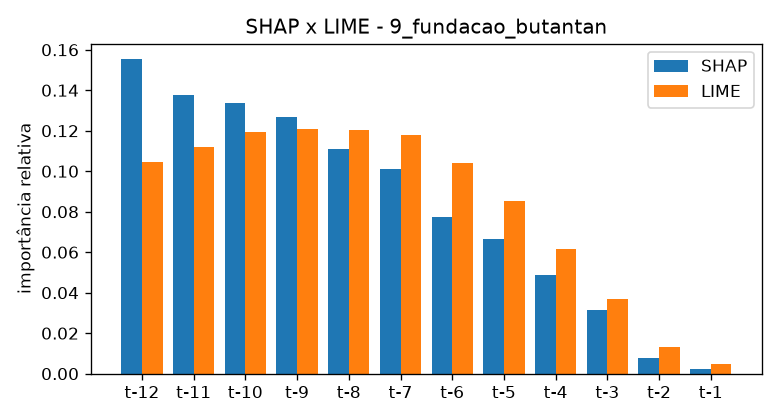
\includegraphics[width=0.78\textwidth]{assets/figures/shap_lime_lag_vac9.png}
  \caption{Importância normalizada por mês da janela (SHAP e LIME), imunobiológico 9 (hepatite B)}
  \label{fig:shap_lime_9}
\end{figure}

\begin{figure}[htb]
  \centering
  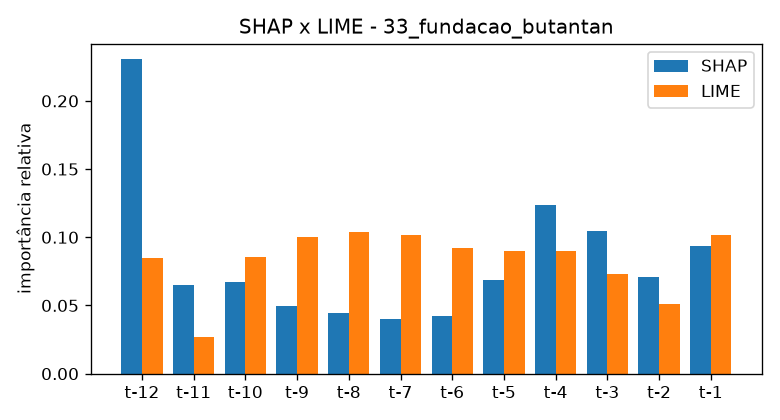
\includegraphics[width=0.78\textwidth]{assets/figures/shap_lime_lag_vac33.png}
  \caption{Importância normalizada por mês da janela (SHAP e LIME), imunobiológico 33 (influenza)}
  \label{fig:shap_lime_33}
\end{figure}

\begin{table}[htb]
  \centering
  \caption{Importância normalizada de meses da janela (modelo apenas com doses, semente 42, 200 amostras de teste)}
  \label{tab:shap_lag}
  \footnotesize
  \begin{tabular}{lcccc}
    \toprule
    \textbf{Imunobiológico} & \textbf{SHAP $t\text{-}12$} & \textbf{LIME $t\text{-}12$} & \textbf{SHAP $t\text{-}1$} & \textbf{LIME $t\text{-}1$} \\
    \midrule
    9 (hepatite B) & 15,5\% & 10,4\% & 0,2\% & 0,5\% \\
    15 (BCG) & 11,2\% & 8,2\% & 0,7\% & 0,6\% \\
    33 (influenza) & 23,0\% & 8,5\% & 9,4\% & 10,1\% \\
    67 (HPV) & 7,9\% & 8,1\% & 4,9\% & 5,2\% \\
    \bottomrule
  \end{tabular}
  \legend{Fonte: Elaborado pelo autor (2026)}
\end{table}

Nos imunobiológicos 9 e 15, SHAP e LIME concordam: a importância decresce dos meses mais antigos para os mais recentes, e o mês imediatamente anterior ($t\text{-}1$) praticamente não pesa (menos de 1\%). O modelo se apoia, portanto, no histórico distante, incluindo o mesmo mês do ano anterior ($t\text{-}12$). No imunobiológico 67, a importância é praticamente plana entre os lags (entre 5\% e 10\%), compatível com um modelo que aprende pouco (melhor época igual a 1 em todas as sementes). No imunobiológico 33, as técnicas divergem: o SHAP concentra 23\% em $t\text{-}12$, enquanto o LIME distribui a importância de forma mais uniforme e atribui 8,5\% a esse lag. Dada a instabilidade do modelo nesse imunobiológico, essa explicação deve ser lida com cautela. Como as amostras explicadas pertencem apenas aos quatro meses de teste, o mapa por mês do calendário cobre uma fração restrita do ano.

\subsection{Extensão com variáveis exógenas}
\label{sec:res_exogenas}

\subsubsection{Desempenho do modelo de referência}

A Tabela~\ref{tab:exogenas} compara o baseline com e sem as nove covariáveis, nas mesmas sementes e no mesmo conjunto de teste. Nos imunobiológicos 9, 15 e 67, as covariáveis não alteram o desempenho: as diferenças de MASE ($-$0,1\%, +0,6\% e $-$0,6\%) ficam dentro de aproximadamente um desvio-padrão entre sementes. No imunobiológico 33, o MASE cai 32\% (de 1,934 para 1,316), o MAE cai 43\% e o desvio entre sementes cai de 0,40 para 0,17. Mesmo assim, o 33 continua acima de 1 e, portanto, não atende ao critério de validação.

\begin{table}[htb]
  \centering
  \caption{Baseline com e sem variáveis exógenas (média $\pm$ desvio-padrão entre cinco sementes)}
  \label{tab:exogenas}
  \footnotesize
  \begin{tabular}{lcccc}
    \toprule
    \textbf{Imunobiológico} & \textbf{MASE sem exógenas} & \textbf{MASE com exógenas} & \textbf{Variação} & \textbf{MAE sem $\rightarrow$ com} \\
    \midrule
    9 (hepatite B) & 0,641 $\pm$ 0,003 & 0,640 $\pm$ 0,003 & $-$0,1\% & 3,10 $\rightarrow$ 2,96 \\
    15 (BCG) & 0,723 $\pm$ 0,016 & 0,727 $\pm$ 0,014 & +0,6\% & 1,64 $\rightarrow$ 1,68 \\
    67 (HPV) & 0,763 $\pm$ 0,009 & 0,758 $\pm$ 0,009 & $-$0,6\% & 2,13 $\rightarrow$ 2,12 \\
    33 (influenza) & 1,934 $\pm$ 0,403 & 1,316 $\pm$ 0,174 & $-$32\% & 100,5 $\rightarrow$ 56,9 \\
    \bottomrule
  \end{tabular}
  \legend{Fonte: Elaborado pelo autor (2026)}
\end{table}

Para os imunobiológicos 9, 15 e 67, três hipóteses, não testadas isoladamente, podem explicar a ausência de efeito: o modelo já aprende pouco, de modo que mais variáveis não rendem sinal; com 12 amostras de treino por município e 120 entradas (10 variáveis por 12 meses), há mais entradas do que dados; e a idade média de uma a três pessoas por mês é basicamente ruído. O imunobiológico 33 é o único com volume suficiente para que as covariáveis de composição carreguem informação, o que é consistente com a melhora observada. Entretanto, essa melhora não foi isolada: pode vir em parte da redução de variância entre sementes. Confirmá-la exigiria um estudo de ablação, removendo uma covariável por vez, ou mais sementes.

\subsubsection{Sensibilidade do modelo com variáveis exógenas}

As Tabelas~\ref{tab:sens_entrada_exo} e \ref{tab:sens_estrutural_exo} repetem a análise de sensibilidade para o modelo com variáveis exógenas, agora para os quatro imunobiológicos. As colunas de baseline são 0,640, 0,727, 1,316 e 0,758, respectivamente.

\begin{table}[htb]
  \centering
  \caption{Sensibilidade do MASE aos parâmetros de entrada (modelo com variáveis exógenas)}
  \label{tab:sens_entrada_exo}
  \footnotesize
  \setlength{\tabcolsep}{3pt}
  \begin{tabular}{llcccc}
    \toprule
    \textbf{Fator} & \textbf{Valor} & \textbf{9 (hep. B)} & \textbf{15 (BCG)} & \textbf{33 (influenza)} & \textbf{67 (HPV)} \\
    \midrule
    Janela & 3 & 0,625 ($-$2,3\%)$^{*}$ & 0,623 ($-$14,4\%)$^{*}$ & 0,773 ($-$41,3\%)$^{*}$ & 0,741 ($-$2,3\%) \\
     & 6 & 0,632 ($-$1,3\%)$^{*}$ & 0,632 ($-$13,1\%)$^{*}$ & 0,860 ($-$34,6\%)$^{*}$ & 0,741 ($-$2,3\%) \\
     & 9 & 0,628 ($-$2,0\%)$^{*}$ & 0,637 ($-$12,4\%)$^{*}$ & 0,806 ($-$38,7\%)$^{*}$ & 0,746 ($-$1,6\%) \\
     & 18 & 0,650 (+1,5\%)$^{*}$ & 0,658 ($-$9,5\%)$^{*}$ & 1,059 ($-$19,5\%) & 0,781 (+3,0\%)$^{*}$ \\
    \midrule
    Ruído & 0,05 & 0,643 (+0,4\%) & 0,729 (+0,2\%) & 1,263 ($-$4,0\%) & 0,759 (+0,1\%) \\
     & 0,1 & 0,644 (+0,6\%) & 0,729 (+0,2\%) & 1,215 ($-$7,6\%) & 0,759 (+0,1\%) \\
     & 0,2 & 0,645 (+0,7\%) & 0,735 (+1,0\%) & 1,385 (+5,3\%) & 0,761 (+0,4\%) \\
     & 0,3 & 0,648 (+1,2\%)$^{*}$ & 0,735 (+1,1\%) & 1,165 ($-$11,5\%) & 0,762 (+0,5\%) \\
    \midrule
    Faltantes & 10\% & 0,638 ($-$0,4\%) & 0,716 ($-$1,6\%) & 1,094 ($-$16,8\%) & 0,755 ($-$0,4\%) \\
     & 20\% & 0,631 ($-$1,5\%)$^{*}$ & 0,700 ($-$3,8\%) & 1,055 ($-$19,8\%) & 0,745 ($-$1,8\%) \\
     & 30\% & 0,620 ($-$3,2\%)$^{*}$ & 0,668 ($-$8,1\%)$^{*}$ & 0,835 ($-$36,5\%)$^{*}$ & 0,716 ($-$5,6\%)$^{*}$ \\
    \bottomrule
  \end{tabular}
  \legend{Fonte: Elaborado pelo autor (2026). $^{*}$ diferença superior a duas vezes o desvio-padrão entre sementes do baseline com exógenas.}
\end{table}

\begin{table}[htb]
  \centering
  \caption{Sensibilidade do MASE aos hiperparâmetros estruturais (modelo com variáveis exógenas)}
  \label{tab:sens_estrutural_exo}
  \footnotesize
  \setlength{\tabcolsep}{3pt}
  \begin{tabular}{llcccc}
    \toprule
    \textbf{Fator} & \textbf{Valor} & \textbf{9 (hep. B)} & \textbf{15 (BCG)} & \textbf{33 (influenza)} & \textbf{67 (HPV)} \\
    \midrule
    Dropout & 0,1 & 0,639 ($-$0,2\%) & 0,718 ($-$1,2\%) & 1,862 (+41,5\%)$^{*}$ & 0,759 (+0,1\%) \\
     & 0,2 & 0,637 ($-$0,5\%) & 0,709 ($-$2,5\%) & 1,644 (+25,0\%) & 0,756 ($-$0,3\%) \\
     & 0,3 & 0,641 (+0,2\%) & 0,712 ($-$2,1\%) & 1,558 (+18,4\%) & 0,753 ($-$0,7\%) \\
    \midrule
    Camadas & 2 & 0,642 (+0,2\%) & 0,720 ($-$1,0\%) & 1,268 ($-$3,6\%) & 0,754 ($-$0,6\%) \\
     & 3 & 0,637 ($-$0,6\%) & 0,712 ($-$2,1\%) & 1,180 ($-$10,3\%) & 0,748 ($-$1,3\%) \\
    \midrule
    Unidades & 16 & 0,646 (+1,0\%) & 0,757 (+4,1\%)$^{*}$ & 1,220 ($-$7,3\%) & 0,768 (+1,2\%) \\
     & 32 & 0,644 (+0,6\%) & 0,745 (+2,5\%) & 1,375 (+4,5\%) & 0,767 (+1,2\%) \\
     & 128 & 0,641 (+0,2\%) & 0,726 ($-$0,2\%) & 1,402 (+6,6\%) & 0,757 ($-$0,1\%) \\
    \midrule
    Taxa de aprend. & $10^{-4}$ & 0,644 (+0,5\%) & 0,722 ($-$0,7\%) & 0,919 ($-$30,2\%)$^{*}$ & 0,767 (+1,1\%) \\
     & $5\times10^{-4}$ & 0,638 ($-$0,3\%) & 0,738 (+1,5\%) & 1,406 (+6,8\%) & 0,766 (+1,0\%) \\
     & $5\times10^{-3}$ & 0,645 (+0,7\%) & 0,726 ($-$0,2\%) & 1,170 ($-$11,0\%) & 0,767 (+1,2\%) \\
    \bottomrule
  \end{tabular}
  \legend{Fonte: Elaborado pelo autor (2026). $^{*}$ diferença superior a duas vezes o desvio-padrão entre sementes do baseline com exógenas.}
\end{table}

O padrão reproduz o do modelo sem exógenas: a janela segue como fator dominante (reduções de 12\% a 14\% no 15 e de 35\% a 41\% no 33 com janelas de 3 a 9 meses), os valores faltantes imputados novamente melhoram o MASE (com 30\%, de 3\% a 8\% nos imunobiológicos 9, 15 e 67 e 37\% no 33), e ruído, camadas e dropout têm efeito pequeno nas séries de baixo volume. Dois resultados são específicos do modelo com exógenas. No imunobiológico 15, 16 unidades pioram o MASE em 4,1\%, único valor com efeito negativo claro, o que sugere que menos unidades limitam a capacidade de aproveitar as 10 variáveis por mês, embora essa leitura seja apenas uma hipótese. No imunobiológico 33, qualquer dropout piorou o MASE (de +18\% a +42\%, com significância apenas em 0,1), ao passo que, sem exógenas, o efeito do dropout nesse imunobiológico não superou o critério de ruído. Note-se que o ruído e os valores faltantes atingem apenas a série de doses, e não as covariáveis.

\subsubsection{Explicabilidade por variável}

A Tabela~\ref{tab:shap_var} apresenta a importância normalizada (SHAP e LIME) das variáveis agregada ao longo dos 12 meses da janela, e a Figura~\ref{fig:shap_var_33} ilustra o caso do imunobiológico 33.

\begin{table}[htb]
  \centering
  \caption{Importância normalizada por variável (modelo com exógenas, semente 42; SHAP / LIME)}
  \label{tab:shap_var}
  \footnotesize
  \setlength{\tabcolsep}{4pt}
  \begin{tabular}{lcccc}
    \toprule
    \textbf{Variável} & \textbf{9 (hep. B)} & \textbf{15 (BCG)} & \textbf{33 (influenza)} & \textbf{67 (HPV)} \\
    \midrule
    Doses aplicadas & 65,4 / 57,3 & 86,6 / 78,7 & 53,4 / 45,6 & 78,2 / 71,6 \\
    Mês sem aplicação & 14,0 / 14,5 & 5,0 / 4,7 & 17,5 / 15,5 & 15,6 / 13,6 \\
    Idade 20 a 59 anos (\%) & 11,0 / 10,6 & 0,3 / 1,1 & 3,9 / 5,4 & 3,9 / 5,3 \\
    Estabelecimento público (\%) & 0,6 / 1,1 & 6,3 / 6,2 & 1,7 / 4,2 & 0,2 / 1,0 \\
    Demais variáveis (soma) & 9,0 / 16,5 & 1,8 / 9,3 & 23,5 / 29,3 & 2,1 / 8,5 \\
    \bottomrule
  \end{tabular}
  \legend{Fonte: Elaborado pelo autor (2026)}
\end{table}

\begin{figure}[htb]
  \centering
  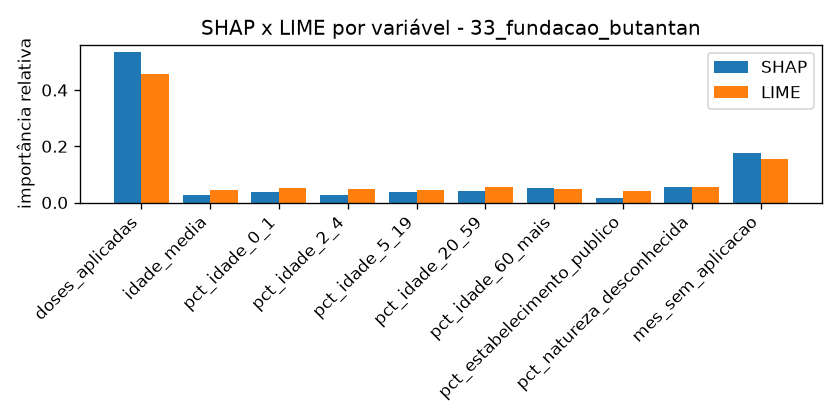
\includegraphics[width=0.85\textwidth]{assets/figures/shap_lime_variavel_vac33_exo.png}
  \caption{Importância normalizada por variável (SHAP e LIME), modelo com exógenas, imunobiológico 33 (influenza)}
  \label{fig:shap_var_33}
\end{figure}

A série de doses passadas é a variável dominante em todos os imunobiológicos, com 53\% a 87\% da importância pelo SHAP. A indicadora de mês sem aplicação é a segunda mais relevante em três dos quatro imunobiológicos (14\% a 18\%; 5\% no 15, onde fica atrás da proporção de estabelecimentos públicos), o que mostra que o modelo usa explicitamente a informação de meses nulos, característica central dessas séries esparsas. As covariáveis demográficas têm importância individual baixa, com duas exceções: a proporção de 20 a 59 anos no imunobiológico 9 (11\%) e, de forma mais distribuída, o conjunto de covariáveis no 33, onde as nove covariáveis somadas respondem por cerca de 47\% da importância, coerentemente com o fato de ser o único imunobiológico em que as exógenas melhoraram o desempenho.

\section{Análise crítica e comparação}

Os resultados mostram um quadro heterogêneo. A LSTM supera o preditor ingênuo sazonal nas três séries de menor volume (MASE de 0,64 a 0,76), mas essa superioridade é modesta e deve ser lida junto com a evidência de que o modelo aprende pouco (melhor época entre 1 e 5, RMSE de validação próximo de 1 e importância SHAP plana ou concentrada em lags distantes). Parte do ganho se explica pela fragilidade do preditor ingênuo em contagens de zero a três doses, estimado com apenas 12 pontos. No imunobiológico de maior volume, o modelo não atinge o critério, e a instabilidade entre sementes (desvio de 0,40 no MASE) é o resultado mais relevante do ponto de vista de risco: duas execuções idênticas, que diferem apenas na semente, podem produzir previsões de qualidade muito distinta.

O uso de SHAP e LIME tornou o comportamento da rede inspecionável: o modelo pesa o histórico distante, inclusive o mesmo mês do ano anterior, o que é plausível para séries com componente sazonal anual, e quase ignora o mês imediatamente anterior nas séries 9 e 15.

Quanto à sensibilidade, o achado mais robusto é o efeito do tamanho da janela, consistente entre imunobiológicos, entre modelos com e sem exógenas e entre critérios de significância. É um resultado com implicação prática direta, pois a janela é uma escolha de projeto de custo nulo. Deve-se, contudo, evitar tratá-lo como prova de que 12 meses é uma escolha ruim por si só: a explicação provável, ainda não testada, é a de mais amostras de treino com janelas curtas. Por outro lado, a robustez ao ruído e à variação de hiperparâmetros nas séries de baixo volume é um resultado favorável à aplicação prática, mas pode refletir justamente o baixo aprendizado do modelo, já que um modelo que pouco extrai da entrada tende a ser pouco afetado por perturbá-la. A melhora com valores faltantes imputados ilustra o cuidado necessário na interpretação: o protocolo mede o erro contra a série original, e a interpolação pode funcionar como suavização.

Por fim, a análise das variáveis exógenas indica que sua utilidade depende do volume: neutras em séries de poucas doses por mês, relevantes para a série de maior volume. Isso sugere que a decisão de incorporar covariáveis demográficas em um sistema real deveria ser tomada por imunobiológico e não de forma uniforme.

\section{Discussão}
\label{sec:discussao}

\textbf{Critério de validação: baseline com MASE inferior a 1.} Atingido em três dos quatro imunobiológicos (hepatite B, BCG e HPV), com margem moderada e com a ressalva de que o modelo aprende pouco; não atingido no imunobiológico de maior volume (influenza), tanto sem exógenas (1,93) quanto com elas (1,32). Portanto, o critério foi atendido parcialmente. Ele é, contudo, um critério fraco: o preditor ingênuo sazonal é estimado com apenas 12 diferenças em contagens de 0 a 3 doses, e a melhor época de validação (1 a 5) e o RMSE de validação normalizado (0,94 a 1,00) indicam que o modelo pouco se afasta da previsão da média. Superar esse preditor não prova que a rede capture a dinâmica da demanda. Baselines mais fortes (último valor, média ou mediana dos últimos 12 meses, médias móveis, ETS, Croston/TSB e um modelo global de gradient boosting) não foram avaliados.

\textbf{Parâmetros de maior influência.} Os parâmetros de maior influência sobre o desempenho foram o tamanho da janela temporal (efeito consistente) e, no imunobiológico de maior volume, a taxa de aprendizado e a presença de dropout no modelo com exógenas; os de menor influência foram o ruído e, nas séries de baixo volume, o número de camadas, de unidades e o dropout.

\textbf{Cenários de maior risco para o planejamento de estoques.} (i) Séries de alto volume e concentradas, em que poucos municípios dominam o erro absoluto (RMSE treze vezes o MAE no imunobiológico 33), justamente aquelas em que um erro de previsão representa mais doses; (ii) janelas longas, que degradam o desempenho; (iii) mudanças de patamar entre treino e teste, como a queda de cerca de metade das doses de influenza em 2026 em relação a 2025, que o modelo não tem como antecipar; e (iv) configurações que, embora pareçam inócuas, são instáveis entre sementes, o que impede confiar em uma única execução.

Um cuidado metodológico precisa ser explicitado: as configurações que levam o imunobiológico 33 abaixo de MASE 1 (janela curta, taxa de aprendizado menor) foram identificadas observando o próprio conjunto de teste. Elas indicam direções promissoras, mas o valor resultante é otimista, e sua confirmação exigiria um conjunto de teste adicional ou a escolha da configuração apenas com base na validação.

% ===============================================================
% CONCLUSÃO
% ===============================================================
\chapter{Conclusão}

\section{Retomada do problema e dos objetivos}

Este trabalho investigou como variações controladas nos parâmetros de entrada e nos hiperparâmetros de um modelo LSTM afetam seu desempenho na previsão mensal de doses aplicadas de quatro imunobiológicos do PNI, por município do estado de São Paulo, e quais entradas mais influenciam as previsões. Os objetivos específicos foram atendidos: construiu-se um pipeline reproduzível de coleta, tratamento e modelagem; treinou-se um modelo de referência com métricas MAE, RMSE, MAPE e MASE; aplicou-se um protocolo de perturbação um fator por vez com cinco sementes, repetido para um modelo com variáveis exógenas; e interpretaram-se os modelos com SHAP e LIME.

O modelo de referência superou o preditor ingênuo sazonal em três dos quatro imunobiológicos (MASE de 0,64 a 0,76) e não o superou no de maior volume (influenza, MASE de 1,93, reduzido a 1,32 com variáveis exógenas). O tamanho da janela temporal foi o fator de maior efeito consistente, com janelas curtas melhorando o desempenho em todos os casos; ruído, dropout, camadas e unidades tiveram efeito pequeno nas séries de baixo volume; e a instabilidade entre sementes dominou o imunobiológico de maior volume. SHAP e LIME mostraram que o modelo se apoia no histórico distante, inclusive no mesmo mês do ano anterior, e pouco no mês imediatamente anterior. Em resposta à pergunta de pesquisa, os resultados não bastam para afirmar que a LSTM seja adequada ao planejamento de estoques de imunobiológicos. Nas séries de baixo volume o modelo supera o preditor ingênuo sazonal, mas esse é um referencial fraco e o modelo pouco se afasta da previsão da média; nas séries de alto volume e sujeitas a mudanças de patamar, o desempenho é instável e não atinge o critério de validação. O que o trabalho estabelece com mais segurança é como o desempenho responde às perturbações, em especial ao tamanho da janela, e que essa resposta depende do volume da série. A adequação da LSTM só poderá ser julgada após a comparação com baselines mais fortes.

\section{Contribuições para a Computação}

A principal contribuição é uma análise sistemática de sensibilidade de uma LSTM aplicada à demanda de imunobiológicos, domínio em que os trabalhos relacionados não submetem o modelo a perturbações controladas na entrada. Contribuem também: (i) a evidência de que, nesse tipo de série curta e esparsa, a escolha da janela temporal pesa mais que os hiperparâmetros estruturais; (ii) a quantificação da variabilidade entre sementes como parte da análise, que distingue o efeito de uma perturbação da sorte de inicialização e revela instabilidade em séries de alto volume; (iii) a aplicação conjunta de SHAP e LIME a uma LSTM nesse domínio, com análise por mês da janela e por variável; e (iv) o pipeline reexecutável, construído sobre dados públicos.

\section{Limitações e trabalhos futuros}
\label{sec:limitacoes}

As principais limitações são:

\begin{enumerate}
    \item \textbf{Séries curtas}: 32 meses por município, o que deixa apenas 12 amostras de treino por município e é o limite principal do trabalho;
    \item \textbf{Teste de quatro meses}, em período de patamar diferente do treino, e uma única partição temporal, sem validação em múltiplas origens;
    \item \textbf{Escopo restrito a São Paulo}: os dados da Bahia, previstos no recorte original, foram coletados, mas não foram incorporados à modelagem, e portanto a comparação entre contextos regionais não foi feita;
    \item \textbf{Esparsidade}: grande proporção de meses nulos e poucas doses por município, o que torna o MAPE pouco informativo;
    \item \textbf{Comparação apenas com o preditor ingênuo sazonal}: não foram avaliados modelos de referência mais fortes (último valor, média ou mediana dos últimos 12 meses, médias móveis, ETS, Croston/TSB, adequado a séries com 25\% a 34\% de meses nulos, e um modelo global de gradient boosting, como o LightGBM), o que torna fraco o critério MASE $<$ 1;
    \item \textbf{Protocolo um fator por vez}, que não captura interações entre fatores, a partir de um único ponto de partida;
    \item \textbf{Valores faltantes e ruído atingem apenas a série de doses}, e a melhora com valores imputados pode ser artefato da suavização;
    \item \textbf{Explicabilidade restrita} à semente 42 e a amostras dos meses de teste;
    \item \textbf{Configurações selecionadas observando o teste}, no caso do imunobiológico de maior volume;
    \item \textbf{Coleta sem tratamento de falhas}, com lacunas em 2021 e 2023 não quantificadas;
    \item \textbf{Hipóteses não testadas}, assinaladas ao longo do texto, como o efeito do número de amostras sobre a janela.
\end{enumerate}

Como trabalhos futuros, sugerem-se: medir o erro por município no imunobiológico de maior volume e testar modelos separados para os municípios de maior porte; realizar um estudo de ablação das covariáveis e ampliar o número de sementes; comparar a LSTM com os baselines mais fortes citados acima, inclusive com um modelo global de gradient boosting; ampliar as séries com mais anos, após corrigir a coleta, e adotar validação em múltiplas origens temporais; testar interações entre fatores com um planejamento fatorial ou busca de hiperparâmetros; investigar o efeito da imputação com outros métodos e com valores faltantes também nas covariáveis; e aplicar o pipeline à Bahia e a outras unidades federativas.

\postextual

% TODO(Gabriel): o TCC1 usava \bibliography{bibliografia}; o template do TCC2 usa
% bibliografia_tcc2. Garanta que este .bib contenha todas as chaves citadas acima.
\bibliography{bibliografia_tcc2}

\end{document}
